% Created 2016-04-01 Fri 12:08
\documentclass{article}
\usepackage[utf8]{inputenc}
\usepackage[T1]{fontenc}
\usepackage{fixltx2e}
\usepackage{graphicx}
\usepackage{longtable}
\usepackage{float}
\usepackage{wrapfig}
\usepackage{rotating}
\usepackage[normalem]{ulem}
\usepackage{amsmath}
\usepackage{textcomp}
\usepackage{marvosym}
\usepackage{wasysym}
\usepackage{amssymb}
\usepackage{hyperref}
\tolerance=1000
\usepackage{minted}
\usepackage{listingsutf8}
\usepackage{enumitem}  %% for lists (in algorithm)
\usepackage{mathtools} %% for \coloneqq
\usepackage{pdflscape}
\usepackage{afterpage}
\usepackage{capt-of}  % or use the larger `caption` package
\usepackage[bottom]{footmisc} %% to keep entire footers on one page
\usepackage[]{graphicx}
\usepackage[]{minted}
\usepackage[a4paper,margin=1in]{geometry}
\usepackage{comment}
\usepackage[linesnumbered,ruled,lined,shortend]{algorithm2e}
\usepackage[space]{grffile}
\setcounter{secnumdepth}{4}
\author{Nicholas Mitchell}
\date{\today}
\title{5\_Empirical\_Studies}
\hypersetup{
  pdfkeywords={},
  pdfsubject={},
  pdfcreator={Emacs 24.5.1 (Org mode 8.2.10)}}
\begin{document}

\maketitle
\tableofcontents

\pagebreak

\section{Empirical studies \label{chapter-empirical-studies}}
\label{sec-1}


\subsection{Financial market data acquisition}
\label{sec-1-1}

Here, a brief summary of the traditional financial data used in this study is presented. Daily data for numerous market segments was collected, using free online sources\footnote{A mixture of \href{http://finance.yahoo.com/}{Yahoo Finance$^{\dag{}}$} and \href{https://www.quandl.com/collections/markets}{Quandl$^{\dag{}}$} was used - please visit them for more information on their original sources. Interfaces were provided by the R packages \href{https://cran.r-project.org/web/packages/quantmod/index.html}{\emph{quantmod$^{\dag{}}$}} and \href{https://cran.r-project.org/web/packages/Quandl/index.html}{\emph{Quandl$^{\dag{}}$}}, respectively.}. Market data is freely available for time-spans that greatly surpass that of Twitter data (and social media data in general\footnote{Market data can be obtained for many indices and assets deep into the last century, whereas social media data older than ten years old is extremely rare.}), which amounts to the fact that the scraped Twitter data is the limiting factor regarding the time-series length used for this study. Table \ref{tab:fin-data} summarises the final market data, categorised by the asset class from which each variable stems. All obtained market data was of daily frequency. The timeline used ranges from 14$^{\text{th}}$ January 2013 until 11$^{\text{th}}$ September 2015, which equates to a total of 971 days, with a total of 695 \emph{weekdays}. The term \emph{weekdays} is intentionally specified, in place of \emph{business days}, as bank holidays in North America remained part of the timeline for modelling\footnote{A detailed listing of the bank holidays can be found in Appendix \texttt{pub-holidays}.}.

A total of seven asset classes were included, covering the majority of traditional stock markets (although futures markets were not included). Options are indirectly incorporated via several indicators for market volatility, e.g. the VIX volatility index (ID 26 in Table \ref{tab:fin-data}) is a metric derived from the implied volatility of highly liquid options\footnote{The exact methods of calculation can be found in the relevant white paper from the \href{https://www.cboe.com/micro/vix/vixwhite.pdf}{Chicago Board Options Exchange$^{\dag{}}$.}}. The single exchange traded fund (ETF) (ID 12) was chosen to represent emerging markets, with the majority of other assets prevalent only in developed economies. The gold and copper spreads (with IDs 27 and 28) were derived as the nominal spread between the spot and three month prices, as a supplementary proxy to short term volatility. The \textbf{Reference} column provides the unique \emph{ticker} or name that is used by the corresponding \textbf{Data Provider}. \emph{Quandl} uses many sources of data (see footnotes for more information), whereas (for this study) the \emph{quantmod} package in R was used as a convenient interface to Yahoo Finance data. In several cases, only one reference is given, which returns the data for several of the variables. For example, all zero-coupon bond data is returned for all maturities from one database call. This is indicated in Table \ref{tab:fin-data} as appropriate.

\begin{table}\
\centering
\begin{tabular}{clllcl}
\textbf{ID} &  & \textbf{Asset class} & \textbf{Asset} & \textbf{Data source} & \textbf{Reference}\\
 &  &  &  &  & \\
\hline
 &  &  &  &  & \\
1 &  &  & Gold spot &  & \texttt{LBMA/GOLD}\\
2 &  &  & Gold 3M &  & (as above)\\
3 &  & Commodities & Copper spot & Quandl & \texttt{LME/PR\_CU}\\
4 &  &  & Copper 3M &  & (as above)\\
5 &  &  & Oil (WTI) &  & \texttt{CHRIS/ICE\_T1}\\
6 &  &  & Natural gas &  & \texttt{OFDP/FUTURE\_NG1}\\
 &  &  &  &  & \\
\hline
 &  &  &  &  & \\
7 &  &  & USD-AUD &  & \texttt{CURRFX/USDAUD}\\
8 &  &  & USD-CAD &  & \texttt{CURRFX/USDCAD}\\
9 &  & Currency pairs & USD-EUR & Quandl & \texttt{CURRFX/USDEUR}\\
10 &  &  & USD-GBP &  & \texttt{CURRFX/USDGBP}\\
11 &  &  & USD-JPY &  & \texttt{CURRFX/USDJPY}\\
 &  &  &  &  & \\
\hline
 &  &  &  &  & \\
12 &  & Exchange traded fund & MSCI Emerging Markets & quantmod & \texttt{EEM}\\
 &  &  &  &  & \\
\hline
 &  &  &  &  & \\
13 &  &  & Zero-coupon 1Y &  & \texttt{FED/SVENY}\\
14 &  &  & Zero-coupon 2Y &  & (as above)\\
15 &  & Fixed income & Zero-coupon 5Y & Quandl & (as above)\\
16 &  & (US bonds) & Zero-coupon 10Y &  & (as above)\\
17 &  &  & Zero-coupon 15Y &  & (as above)\\
18 &  &  & Zero-coupon 20Y &  & (as above)\\
 &  &  &  &  & \\
\hline
 &  &  &  &  & \\
19 &  &  & DAX          (Germany) &  & \texttt{\textasciicircum{}GDAXI}\\
20 &  &  & Dow Jones    (U.S.) &  & \texttt{\textasciicircum{}DJI}\\
21 &  & Stock indices & FTSE100      (U.K.) & quantmod & \texttt{\textasciicircum{}FTSE}\\
22 &  &  & Nikkei 225   (Japan) &  & \texttt{\textasciicircum{}N225}\\
23 &  &  & S\&P500       (U.S.) &  & \texttt{\textasciicircum{}GSPC}\\
24 &  &  & Shanghai SE  (China) &  & \texttt{000001.SS}\\
 &  &  &  &  & \\
 &  &  &  &  & \\
\hline
 &  &  &  &  & \\
25 &  &  & VXD (Dow Jones) &  & \texttt{CBOE/VXD}\\
26 &  & Volatility indicators & VIX (S\&P500) & Quandl & \texttt{YAHOO/INDEX\_VIX}\\
27 &  &  & Gold spread &  & (derived)\\
28 &  &  & Copper spread &  & (derived)\\
 &  &  &  &  & \\
\hline
 &  &  &  &  & \\
\end{tabular}\caption[A breakdown of all financial market data used]{\label{tab:fin-data}A summary of the financial market data to be paired with sentiment analysis results. Daily frequency was obtained for all data, meaning no interpolation was necessary. Imputation was performed using the LOCF method.}

\end{table}


\subsection{Data preparation \label{data_prep}}
\label{sec-1-2}


\subsubsection{Data transformations \label{data-trans}}
\label{sec-1-2-1}

The combined output of Chapters \texttt{chapter-twitter-mining} and \texttt{sentiment-analysis-chapter} consists of the sentiment of individual tweets for each of the thirteen search terms over a two year eight month period. This forms one half of the data set to be used, which necessitated further manipulation before being combined with financial market data for modelling. Aggregating to daily frequency was a requirement, and there were several ways to to do this. This following sub-sections outline how this was achieved.


\paragraph{Re-scaling sentiment scores \label{rescaling-sent}}
\label{sec-1-2-1-1}

The results that were returned from the five sentiment analysis models (at the individual tweet level) were all on slightly different scales. Although within the same orders of magnitude, $\pm 10$, they were re-scaled to be spread over the same range for consistency's sake. This also facilitated the combination of data from the different models, as discussed in the Section \ref{combined-sent}. When re-scaling the sentiment scores, it was important to retain the meaning that the scores conveyed, i.e. a positive value conveyed a positive sentiment, and vice versa. Therefore it was not an option to simply normalise the data, giving it a mean value of zero and a desired variance, as this would have inevitably meant that some individual scores would cross the \emph{zero-boundary}, thereby changing their sign and losing their true meaning. The method that was therefore used, was to merely reduce their magnitudes, so that the maximum score within one set of tweets\footnote{One set signifies the tweets for one search term, for one sentiment analysis model. Thirteen search terms and five models gave sixty-five initial data sets.} was equal to one. This was achieved by simply dividing the scores for each data set by the maximum scores in that set. In the special case of the SentiStrength data, which produces a binary output, the two response were first averaged - creating a single score for each tweet - before being re-scaled to the same range as the other sentiment scores: $[-1, 1]$.


\paragraph{Weighted aggregation of sentiment scores \label{weighting-sentiment}}
\label{sec-1-2-1-2}

The second form of aggregation that was necessary to perform on the Twitter data, was to ensure that each of the thirteen search terms provided a \emph{single} score for each day (from each of the five sentiment models). This aggregation was a necessary step to match the frequency of the financial market data. In this step, the additional meta data that was \emph{scraped} for each tweet was brought into use. Instead of computing the average score for each day over all tweets, each tweet's individual score was first weighted, by using both the number of times that it was \emph{retweeted} as well as the number of times it was marked as a \emph{favourite} by another user. The reasoning behind this step may be explained as follows: if one tweet has a score of e.g. $+2$, this means one person has a positive sentiment concerning the matter that was tweeted. If then five additional people retweeted or favourited that tweet, they thereby show their agreement with that tweet, and so the underlying sentiment is magnified in its interpretation. Therefore, a tweet that has been retweeted and favourited many times should logically carry more weight into the required average for that day, as it represents the opinion of a greater number of people. Let a \emph{tweet event} be defined as one additional opinion, i.e. one retweet or one marking as a favourite. Given this, the methodology used for weighting a single tweet may be summarised as follows:

\begin{equation}
  score_{weighted} = \left( \frac {\tau }{ \sum_{i = 1}^{N} \tau_{i} } \right) \cdot score_{original}
  \label{eqn-reweight}
\end{equation}

\vspace{3mm}

where $\tau$ is the total events for the tweet being weighted and $N$ is the number of tweets on the day in question. This means the denominator represents the total sum of tweet events on that day, for that specific search term. Using this, the sentiment score for each day reflects the sentiment found on Twitter with an added amount of precision.


\subsubsection{Imputation \label{imputation}}
\label{sec-1-2-2}

As was touched upon in Section \texttt{final-output}, there was a negligible proportion of missing data in the sentiment analysis results (< 1 \%). The majority of missing data, throughout both the financial market and sentiment analysis data sets (weekends having been removed) could be contributed to public holidays. As the vast majority of the data listed in Table \ref{tab:fin-data} was obtained from American markets, only official public holidays from America were considered. Over the 695 period timeline there were a total of 25 public holidays ($\approx$ 3.6 \% of the periods), which are detailed in Table \texttt{tab:public-holidays}, Section \texttt{pub-holidays}. The weekends were removed from the sentiment analysis data, in order to be combined with the market data.

Even though the percentage of missing data within the entire data set (including sentiment data and market data) fell below 1 \% after removing weekends, the component-wise boosting models do not (by default) tolerate missing data. Therefore it was necessary to use a method of imputation; the method selected was that of \emph{last observation carried forward} (LOCF). This must be carried out before the log-returns are computed\footnote{Otherwise the result from that computation would be twice as many missing data points, when using the \texttt{diff()} function within R.}. Using LOCF implies then that the log-return is simply equal to zero on days where no data was received, as the difference would be zero between the imputed day and its preceding day. Additionally, imputing the data instead of removing the data was not able to create a large bias, as there are so few missing data points. Other methods of imputation that were considered include splines, k-Nearest Neighbour and variable modelling\footnote{This involves modelling each individual variable in a way that allows one to impute the variable using its own distribution.}; however, as the proportion of missing data was so low, these more complicated methods were not warranted. As the public holidays were imputed, a dummy variable was created to make use of the information, if possible\footnote{See Section \ref{dummy-vars}, where the inclusion of public holidays and other deterministic factors were included in the model.}.


\subsubsection{Derived variables}
\label{sec-1-2-3}


\paragraph{Weekend sentiment \label{weekend-sent}}
\label{sec-1-2-3-1}

The sentiment analysis data was collected over a total of 971 days, in continuous time, without any breaks. This means there was sentiment data available from the weekends that could not be directly modelled alongside market data, which is only for weekdays. In an attempt to capture sentiment from the weekend, a new variable was created that incorporated sentiment data from each weekend, and was used in modelling the following Monday's returns\footnote{This variable was constructed out of the intuition that it makes sense that sentiment scores from the weekend should reflect the opinions of people who may make trades on the following Monday. However, no thorough statistical analysis was performed in the construction of this new variable.}.

In order to extract the weekend sentiment, the values from each Friday, Saturday and Sunday were grouped into one mean value, which replaced the original value for the same Friday\footnote{One could imagine a more complicated method of combining the sentiment scores for future work. For example, it is theoretically possible to weight the tweets, giving more weight to those closer to the Monday, to reflect a belief that \emph{younger} sentiment scores reflect more relevant opinions, and so exponential smoothing could be used, for example.}. This final Friday value was the value to be used in predicting the next day, i.e. the immediately following Monday. By not using any information at or further ahead of in time than the outcome variable, there is no violation of temporal information flow. For this new variable, only three of the thirteen search terms were selected; "Dow Jones", "federal reserve" and "stock prices". This is because the interpretation regarding the underlying sentiment becomes rather difficult once more are combined. The three terms were chosen due to their obvious correlation in underlying sentiment with market movements. Figure \ref{fig:wwp} illustrates the combined sentiment score of the newly derived variable against movements of the DJIA - the weekends are shaded, and the lack of market data is noticeable by zero returns on the shaded regions. It can be observed that the movement of the sentiment over the weekend coincides with a market movement in the same direction for the second and third of the three weekends. Furthermore, it can be seen that the sentiment rises over all three Mondays (the segments directly following the shaded regions), which reflects the market movements on the first Monday and precedes the Market's actual upwards movement in the second and third weeks.

\begin{figure}[htb]
\centering
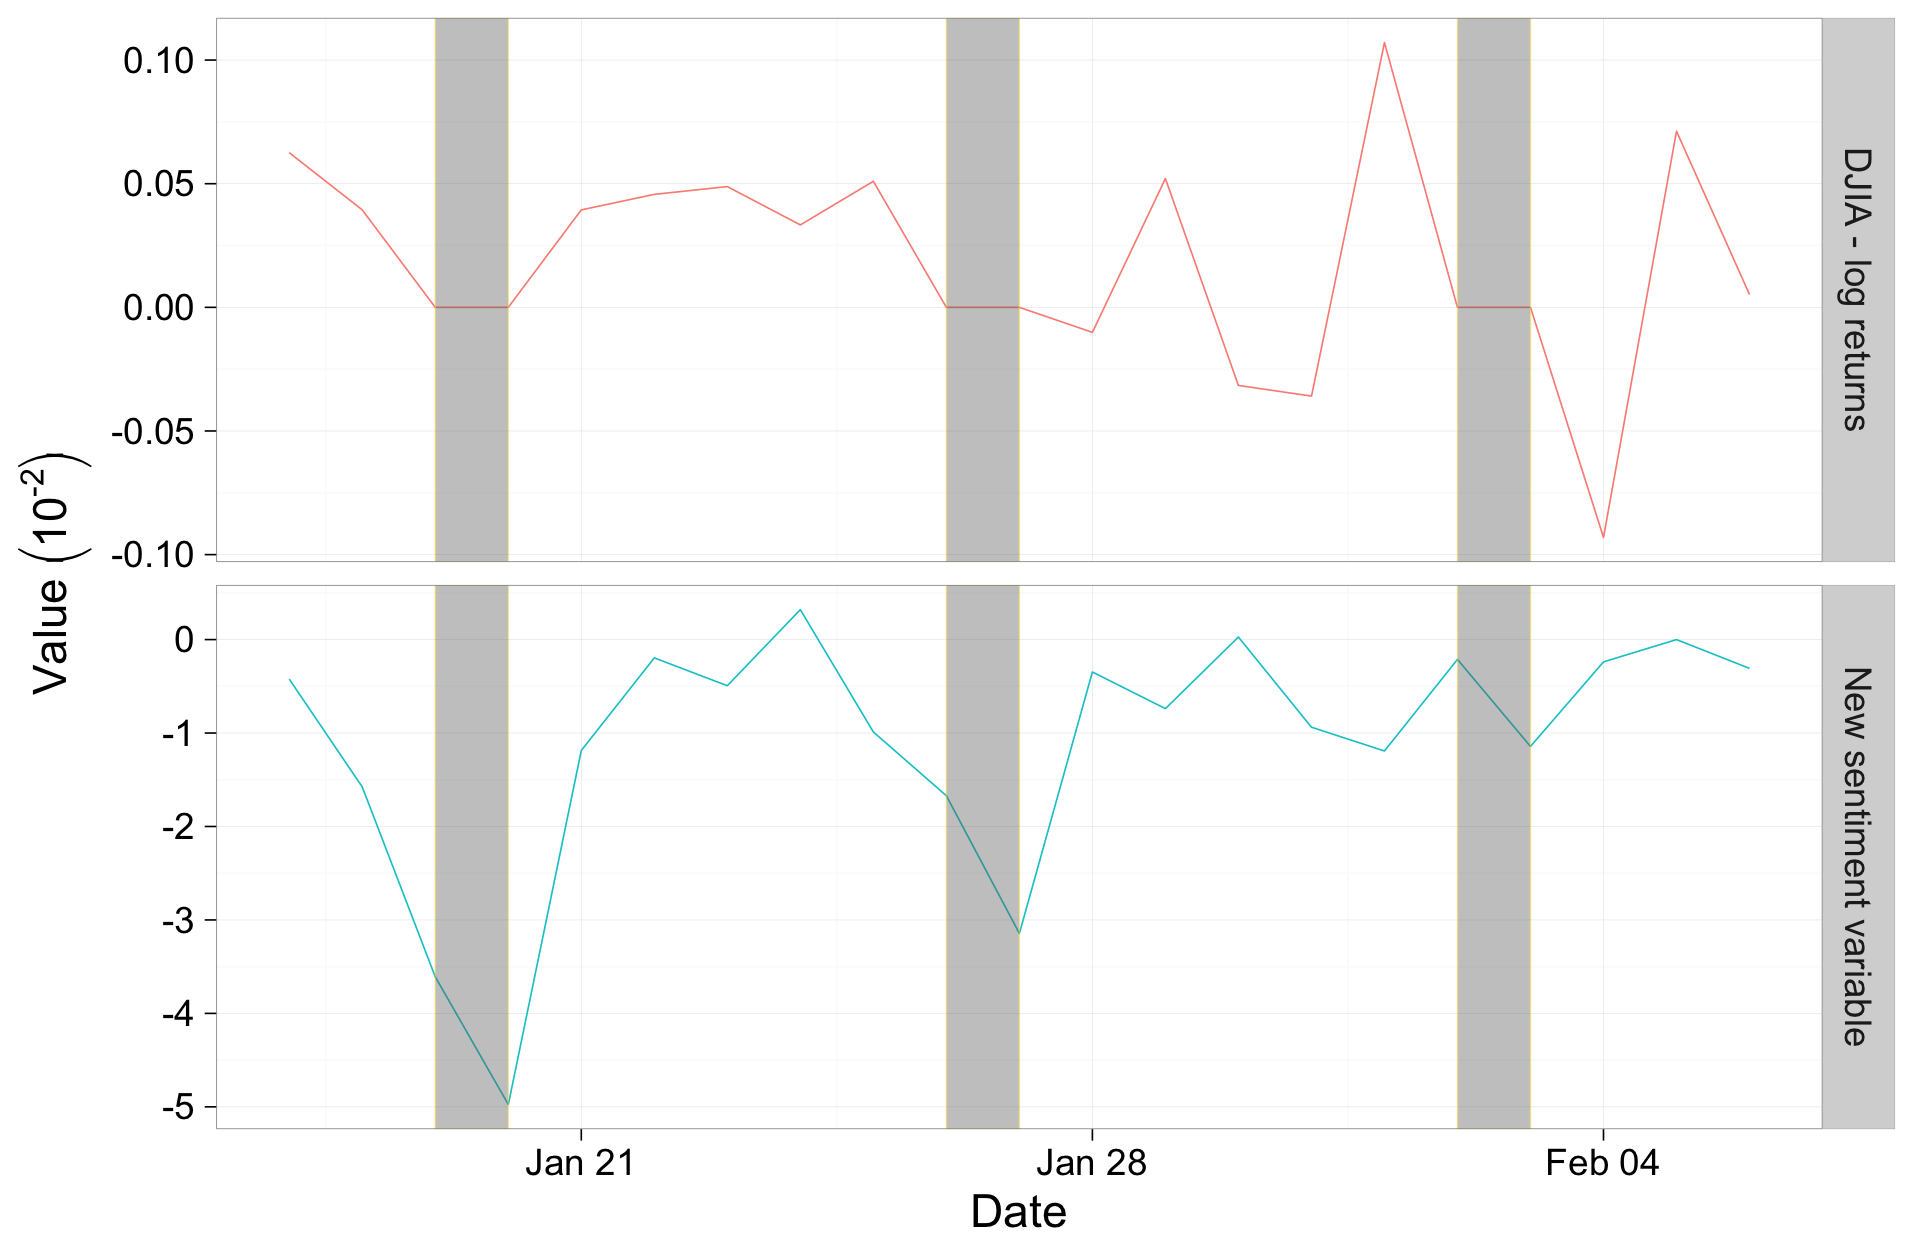
\includegraphics[width=16cm]{/Volumes/Mac OS Drive/Thesis/Source Code/Reporting/nwm_Report/images/weekend_sentiment_variable.png}
\caption[An illustration of weekend sentiment as a predictor]{\label{fig:wwp}A comparison between the derived weekend sentiment variable (an average of three single sentiment variables) against the log returns of the DJIA. Dates are taken from 2013, with weekends highlighted by grey rectangles.}
\end{figure}


\paragraph{Combined sentiment models \label{combined-sent}}
\label{sec-1-2-3-2}

As mentioned above, five sentiment analysis models were used to score the tweets. A last set of variables were created in order to condense the sentiment data into fewer variables. This was performed simply by using the mean over all five sentiment analysis models, for each of the thirteen search terms. These variables were used in the creation of more succinct data sets, which can be seen and compared to the other in Section \ref{subsets}.


\paragraph{Dummy variables \label{dummy-vars}}
\label{sec-1-2-3-3}

Certain facets of time-series data are deterministic: these dummy variables relate to the days of the week. Two dummy variables (DVs) were created in the hope that the component-wise boosting methodology would be able to use them; at the same time knowing, however, that they would not be promoted by the model if no effect was noticeable due to their inclusion. Both DVs relate to days and dates, with the first returning either a 1 or 0, stating whether the day is a Monday or not, respectively. The second DV answers a similar question, making use of the known public holidays (as discussed in Section \ref{imputation}), stating simply whether a day was a public holiday or not.

When creating the lagged variables for each data set (described in Section \ref{lagged-subsets}), these two DVs were able to, additionally, be included alongside the outcome variable, without being lagged. This is because, if it is believed that stocks perform badly on Mondays, it is known in advance that Monday is coming and so traders may adjust their strategies accordingly. The information is deterministic. For more ideas into the realm of deterministic cyclic trading patterns, see \cite{gondhalekar2003blue} and \cite{kamstra2003winter}.


\subsubsection{Final subsets for comparative modelling \label{subsets}}
\label{sec-1-2-4}

The last step in data pre-processing was to organise the data in a way that allowed a direct measure of the benefit that adding sentiment data to market data supplied. To do this, five data sets were defined - their names, contents and reasoning are explained in Table 6. The data sets displayed were then later increased in size when predictor variables were lagged. The largest data set was the \emph{combined} data set, with 693 predictor variables, which is two greater than the number of observations, 691\footnote{Without any lagged variables, the timeline includes 695 days; however, when creating lagged variables, the timeline is reduced in length by one day for each additional lag.}.

\afterpage
\clearpage
\thispagestyle{empty}
\begin{landscape} \hspace{1pt}
\centering

\begin{center}
\begin{tabular}{lllclll}
 &  &  &  &  &  & \\
 & \textbf{Subset name} &  & $\sum$ &  & \textbf{Contents} & \textbf{Reasoning}\\
 &  &  &  &  &  & \\
\hline
 &  &  &  &  &  & \\
 &  &  &  &  & A selection of six of market data variables: & A benchmark model that should perform satisfactorily,\\
 & traditional$_{\text{small}}$ &  & 6 &  & S\&P500, gold (spot), oil, USD-EUR, and & and allow for fair comparison with fitting methods\\
 &  &  &  &  & 1o year zero-coupon bond yield & that do not have inherent method of variable selection.\\
 &  &  &  &  &  & \\
\hline
 &  &  &  &  &  & \\
 &  &  &  &  & All market data, as listed in Table \ref{tab:fin-data}, & To combine and showcase component-wise boosting,\\
 & traditional$_{\text{large}}$ &  & 36 &  & plus dummy variables (Section \ref{dummy-vars}) & being able to select the strongest candidates for\\
 &  &  &  &  &  & a model with traditional predictors.\\
 &  &  &  &  &  & \\
\hline
 &  &  &  &  &  & \\
 &  &  &  &  & Sentiment results for each search term & A compact collection of the sentiment analysis results.\\
 & sentiment$_{\text{small}}$ &  & 22 &  & averaged over the five sentiment models, & as with traditional$_{\text{small}}$, a benchmark model to show the\\
 &  &  &  &  & plus dummy variables (Section \ref{dummy-vars}) & predictive power of sentiment scores by themselves.\\
 &  &  &  &  &  & \\
\hline
 &  &  &  &  &  & \\
 &  &  &  &  & All sentiment results: each search & To allow boosting to select the very best components\\
 & sentiment$_{\text{large}}$ &  & 100 &  & term passed through each sentiment model, & of the sentiment analysis results. Also to facilitate\\
 &  &  &  &  & plus dummy variables (Section \ref{dummy-vars}) & direct comparisons to the combined data set.\\
 &  &  &  &  &  & \\
\hline
 &  &  &  &  &  & \\
 &  &  &  &  & All variables: the summation of traditional$_{\text{large}}$, & To demonstrate the effect of combining sentiment\\
 & combined &  & 142 &  & sentiment$_{\text{small}}$ and sentiment$_{\text{large}}$, & analysis results with traditional market data. A large\\
 &  &  &  &  & plus dummy variables (Section \ref{dummy-vars}) & data set, exploiting the model's variable selection.\\
 &  &  &  &  &  & \\
\hline
\end{tabular}
\end{center}

\captionof{table}[The descriptions of the five base subsets used for comparisons]{The five different subsets created from the financial market and sentiment analysis data. The subset names, total number of variables $\left( \sum \right)$, a summary of the constituents as well as a description of each data set is given. The last column, Reasoning, explains how the subsets were chosen to (1) demonstrate the ability of component-wise boosting, (2) to highlight the impact of social media data on predictive accuracy, and (3) to allow for comparisons to other models.}\label{tab_subsets}
\end{landscape}
\clearpage


\paragraph{Lagged subsets \label{lagged-subsets}}
\label{sec-1-2-4-1}

After the five different subsets were defined, several variations were made for each of them to include lagged predictor variables. For each of the subsets, four additional subsets were created, including lags of two to five with respect to the outcome variable; the DJIA. Each further degree of lagged variables was appended to the previous lagged subset. Using a fictional data set with a univariate outcome, $y$, and only one predictor, $x$, the resulting five subsets (including the base) may be illustrated as follows:

\begin{center}
\begin{tabular}{lll}
 &  & \\
\textbf{Base subset:} &  & $y_t = x_{t-1}$\\
 &  & \\
\textbf{Second lag:} &  & $y_t = x_{t-1} + x_{t-2}$\\
 &  & \\
\textbf{Third lag:} &  & $y_t = x_{t-1} + x_{t-2} +x_{t-3}$\\
 &  & \\
\textbf{Fourth lag:} &  & $y_t = x_{t-1} + x_{t-2} +x_{t-3} +x_{t-4}$\\
 &  & \\
\textbf{Fifth lag:} &  & $y_t = x_{t-1} + x_{t-2} +x_{t-3} +x_{t-4} +x_{t-5}$\\
 &  & \\
\end{tabular}
\end{center}


where intercepts and parameter coefficients have been omitted for simplicity. This was performed for each of the five subsets defined in Section \ref{subsets}, which means a total of 25 sets of data were defined. Each of these subsets was used for each of the parameter configurations within the component-wise boosting modelling phases - for more information, refer to Section \ref{main-modelling}.


\subsubsection{Pairwise correlation reduction \label{pairwise-corr}}
\label{sec-1-2-5}

As was discussed within Chapter \texttt{chapter-gradient-boosting}, the variable selection ability of component-wise gradient boosting does have limits. If two variables are highly correlated and so produce similar approximations to the negative gradient of the loss function, the model will have no way to really distinguish exactly which is the best. In such a case, this would lead to almost random selection between the two variables. In order to minimise the likelihood of this occurring during the modelling, as well as to improve the numerical stability of the gradient descent, a method to remove correlation within the data sets was devised; specifically, pairwise correlation was targeted. 

The method used to purge pairwise correlation from the data set is detailed by Algorithm \eqref{alg-corr-cutoff}. The removal of variables was performed iteratively, re-calculating the remaining correlation within the data set after each individual variable was removed. This method presents a more systematic means of removing only those variables, which may impede the overall performance within the boosting procedure, described in Section \texttt{comp-alg}.

\vspace{5mm}

\begin{algorithm}[H]
  \caption{Iteratively removing pairwise correlation within a data set}
  \label{alg-corr-cutoff}

  \BlankLine
  \BlankLine

  \SetKw{Return}{return} %% Custom keyword
  \KwIn{correlation matrix of data set, $\mathcal{C} $; maximum allowed pairwise correlation, $\kappa$ }
  \KwOut{data set with reduced pairwise correlation}
  
  \BlankLine
  \BlankLine
  
  \While{ \hspace{3mm} $\max \mathcal{C} > \kappa $ \hspace{3mm} }{
    \BlankLine
    \begin{enumerate}[leftmargin=12.5mm]
      \BlankLine
    \item [Step 1.] Identify the two variables exhibiting the highest pairwise correlation 
    \item [Step 2.] Compute which has the greatest cumulative pairwise correlation over the entire data set
    \item [Step 3.] Remove this variable from the pair  
    \item [Step 4.] Re-calculate the correlation matrix, having removed one variable
    \end{enumerate}
  }

  \BlankLine
  \Return{data set with $\max \mathcal{C} \leqslant \kappa$}
\end{algorithm}

\vspace{5mm} 

The maximum level of correlation, $\kappa$, to choose for each model is not something that can be analytically decided upon. Depending on the levels chosen, the number of variables that are removed from a data set can change rather drastically. Figure \ref{fig:corr-cutoff} illustrates the number of variables that are removed from both the \emph{traditional$_{\text{large}}$} and \emph{combined} data sets, as a function of the correlation threshold, $\kappa$. The left y-axis shows the number of predictors that are removed for a given $\kappa$, whereas the right y-axis shows that number as a percentage of the total number of predictors in that data set. The error bars highlight how many predictors are removed as $\kappa$ crosses that specific threshold (reading $\kappa$ from low to high). It can be seen that, even choosing a relatively high value for $\kappa$, e.g. $\approx$ 80 \%, removes approximately 25 \% of predictors for the \emph{traditional$_{\text{large}}$} data set, whereas more than 35 \% of predictors are removed from the \emph{combined} data set at the same level of $\kappa$. This shows that the level of correlation within the \emph{combined} data set is larger than that of the (smaller) \emph{traditional$_{\text{large}}$} data set. This might be expected, as the \emph{combined} data set contains e.g. five values (and so five predictors) of sentiment for each search term, one for each sentiment model - these should be highly correlated by nature.

As is outlined in Section \ref{param-grid}, a selection of threshold values, $\kappa$, were used for modelling, meaning the effect of correlation within the data is able to be considered when inspecting the collated results. Both of the curves in Figure \ref{fig:corr-cutoff} are approximately linear. In the case of the \emph{traditional$_{\text{large}}$} data set, one may loosely keep in mind that the value of $\kappa$ roughly equates to the percentage of original predictors that remain in the data set for modelling.

\begin{figure}\
\centering
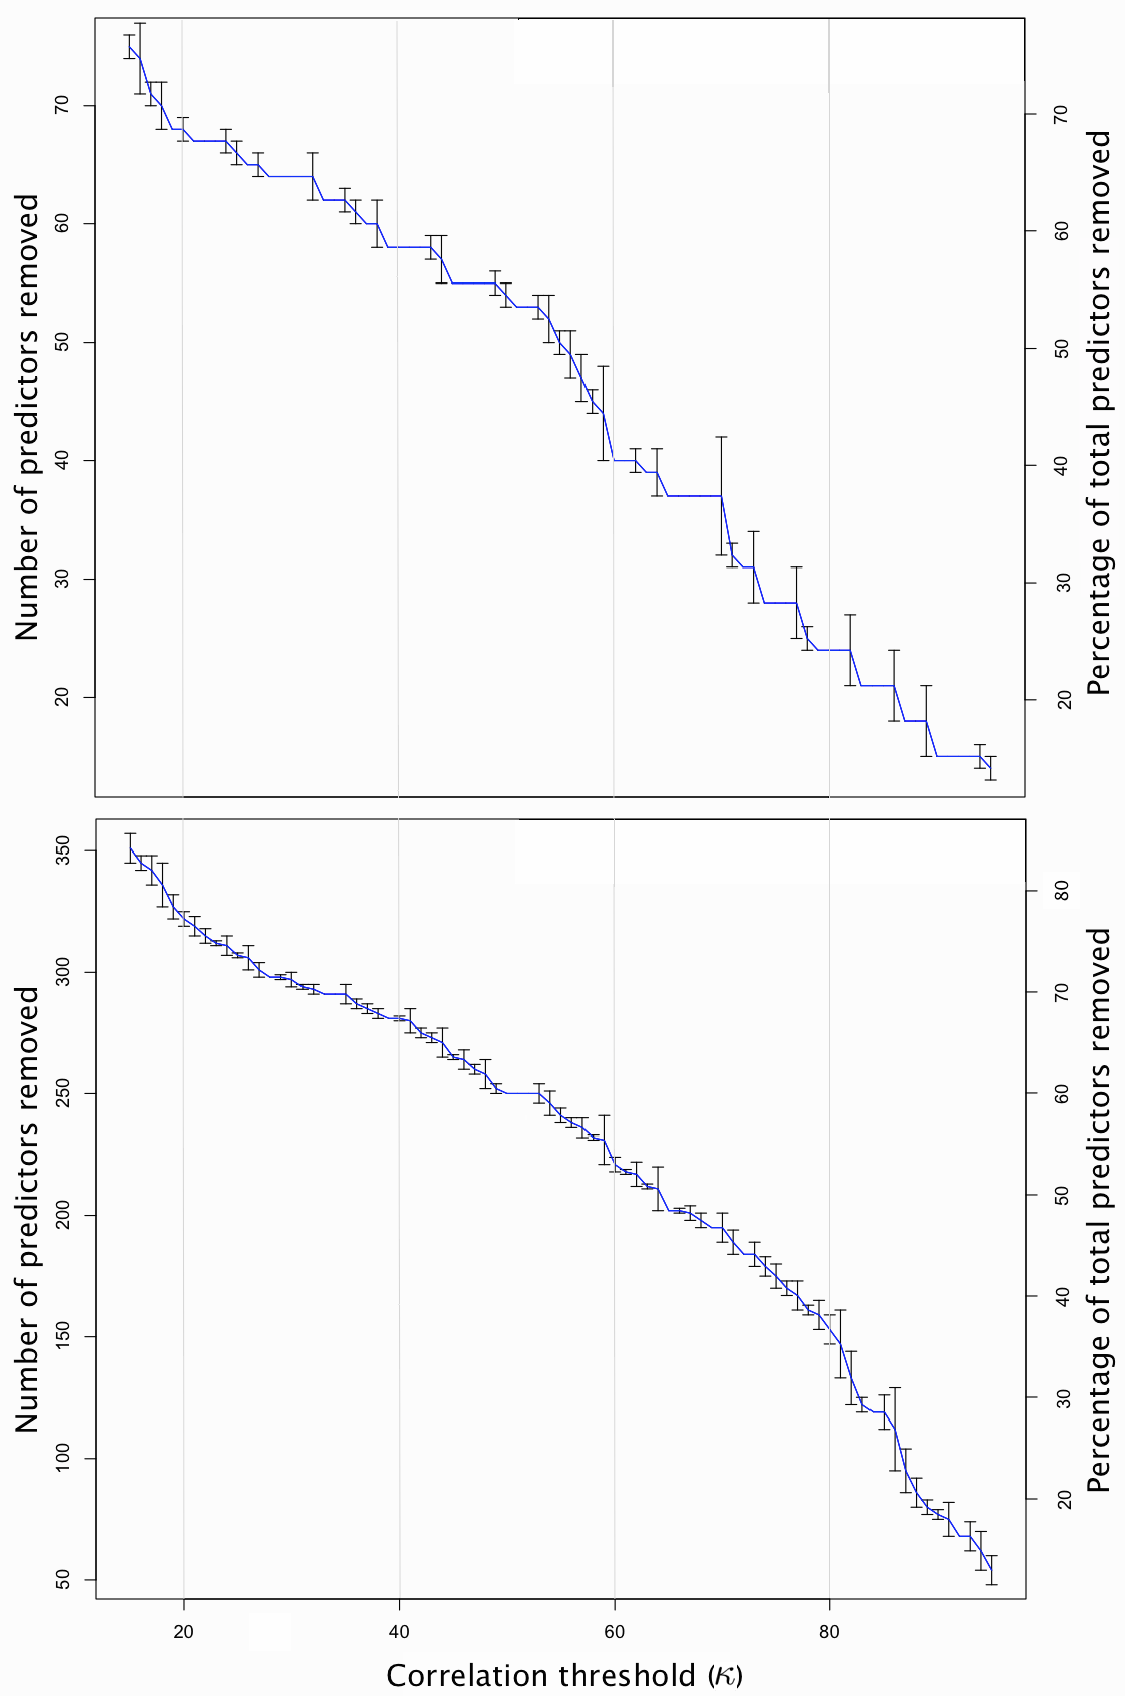
\includegraphics[width=14cm]{/Volumes/Mac OS Drive/Thesis/Source Code/Reporting/nwm_Report/images/corr-cutoff-mixture.png}
\caption[The number of predictors removed as a function of the correlation threshold, $\kappa$]{\label{fig:corr-cutoff}The number of predictors that are removed as a function of the correlation cutoff, $\kappa$. (Top) the \emph{traditional$_{\text{large}}$} data set with three lags; (bottom) the \emph{combined} data set with three lags. The vertical bars placed along the curve reflect how many predictors are removed for the corresponding value of $\kappa$.}
\end{figure}


\pagebreak


\subsection{Data exploration \label{data-exploration}}
\label{sec-1-3}

Before modelling commenced, the obtained, cleaned and collated data was explored and visualised in order to better understand the structure, and perhaps to gain some insights that may help with making modelling decisions as well as interpreting results. The main outcomes are presented here, allowing the reader to become acquainted with the data set. As the social media data and the sentiment analysis thereof is the novel segment, which this study aims to leverage, the presentation of the data will focus on this area, as well as its relationship to features of the outcome variable: the Dow Jones Industrial Average (DJIA) stock index.


\subsubsection{Macro view with examples \label{macro-view}}
\label{sec-1-3-1}

\begin{wrapfigure}{l}{0.5\textwidth}
\centering
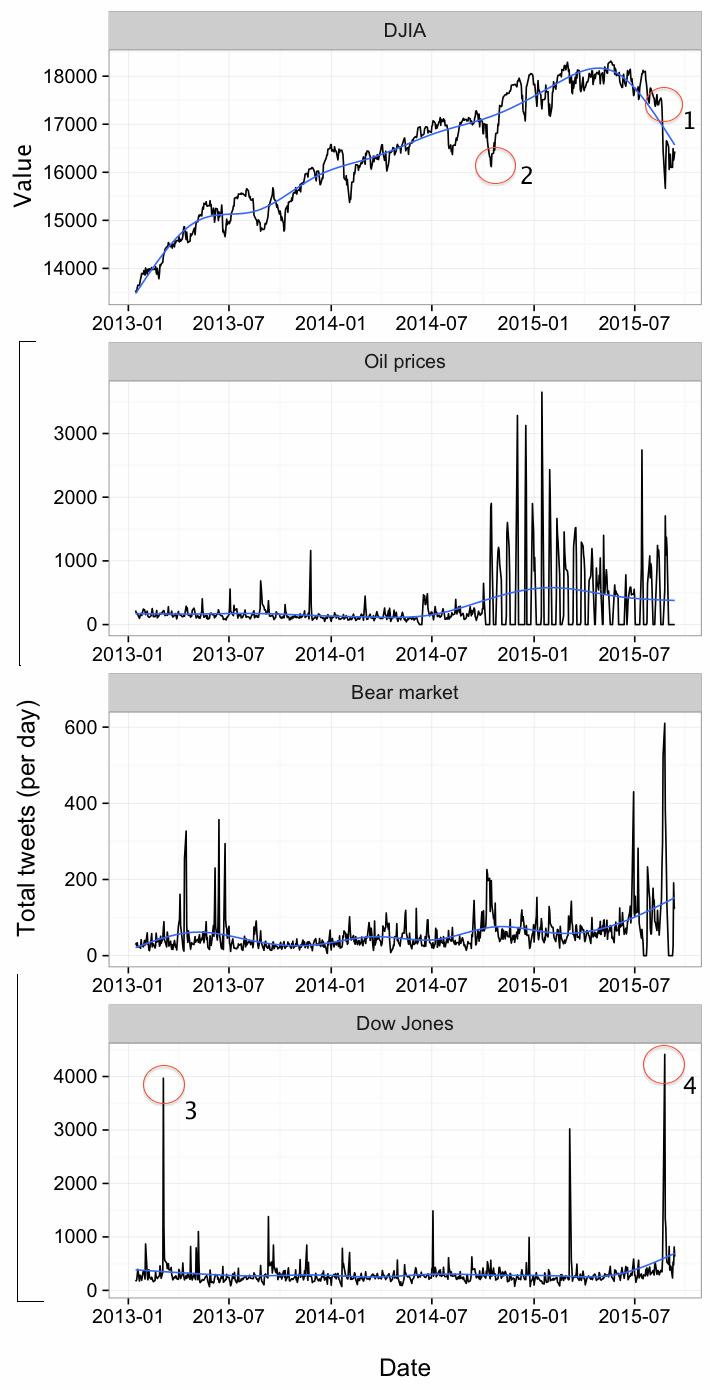
\includegraphics[width=0.48\textwidth]{/Volumes/Mac OS Drive/Thesis/Source Code/Reporting/nwm_Report/images/tweet-counts-facet.png}
\caption[Movements of the DJIA compared to Twitter activity]{\label{fig:tweet-counts-facet}Individual plots for the DJIA and the tweet counts of three search terms (given in the facet titles), plotted over the entire time, each with a blue trendline. Several key events are highlighted and numbered.}
\end{wrapfigure}

As was presented in Section \texttt{final-output}, the total number of tweets obtained from Twitter was 2,350,217. Figure \ref{fig:tweet-counts-facet} gives a facet view of how the tweets for several of the thirteen search terms are dispersed over the timeline\footnote{The tweet data is aggregated to daily sums of tweets - see Section \ref{data-trans} for more information.}, i.e. \hspace{-12pt} the frequency with which the search terms appeared on Twitter. The blue line on each of the facet plots highlights the trend for that given variable, several points of interest are highlighted with red circles. The DJIA rises for the majority of the timeline, until it plateaus at the end of 2014, with a free-fall drop (labelled "1") at the end of summer 2015. An interesting correspondence is that between the astonishing increase in "oil prices" tweets, just \textbf{before} the DJIA takes a short dip and begins to plateau (labelled "2"). Additionally, the number of tweets containing "bear market" begins to rise almost a month before the sharp fall (marked "1").
The two circles peaks (labelled "3" and "4") on the bottom facet more than likely signify reactionary tweets to extraordinary market movements. The first can be traced to 28$^{\text{th}}$ March 2013, where the DJIA closed at a \href{http://www.ibtimes.com/sp-500-dow-jones-industrial-average-stock-indexes-close-record-high-markets-recovery-1153105}{record high$^{\dag{}}$}. The circled peak "4" clearly aligns with circle "1", on 24$^{\text{th}}$ August 2015, on which day the DJIA plummeted over 1,000 points on \href{http://www.ibtimes.com/dow-jones-industrial-average-plummets-global-stocks-take-black-monday-plunge-great-2065359}{negative news$^{\dag{}}$} regarding China's economy. These signs illustrate that there is a two-way relationship between the movements of the DJIA and the activity on Twitter. Some larger trends seem to be visible through the number of tweets (and likely through the resulting sentiment scores), whereas other features highlight purely the reactive nature of Twitter users to market events. It is the former, which the modelling is aimed at exploiting; the periods of momentum ought to be captured. How this is targeted is discussed further in Section \ref{param-grid}.


\subsubsection{Micro view \label{micro-view}}
\label{sec-1-3-2}

The previous section showed large peaks in the tweet count at potentially important events in the markets timeline; however, here a closer look is taken at the same relationship by inspecting the day-to-day movements of the market versus the activity on Twitter. Figure \ref{fig:day-to-day} shows the relationship between the DJIA, log returns thereof and number of tweets computed using tweets containing "Dow Jones". The level of correlation between the log returns and the Twtter data are clear, with moves in Twitter data reflecting, and in the days immediately following 16$^{\text{th}}$ February, preceding those of the market.

\begin{figure}[htb]
\centering
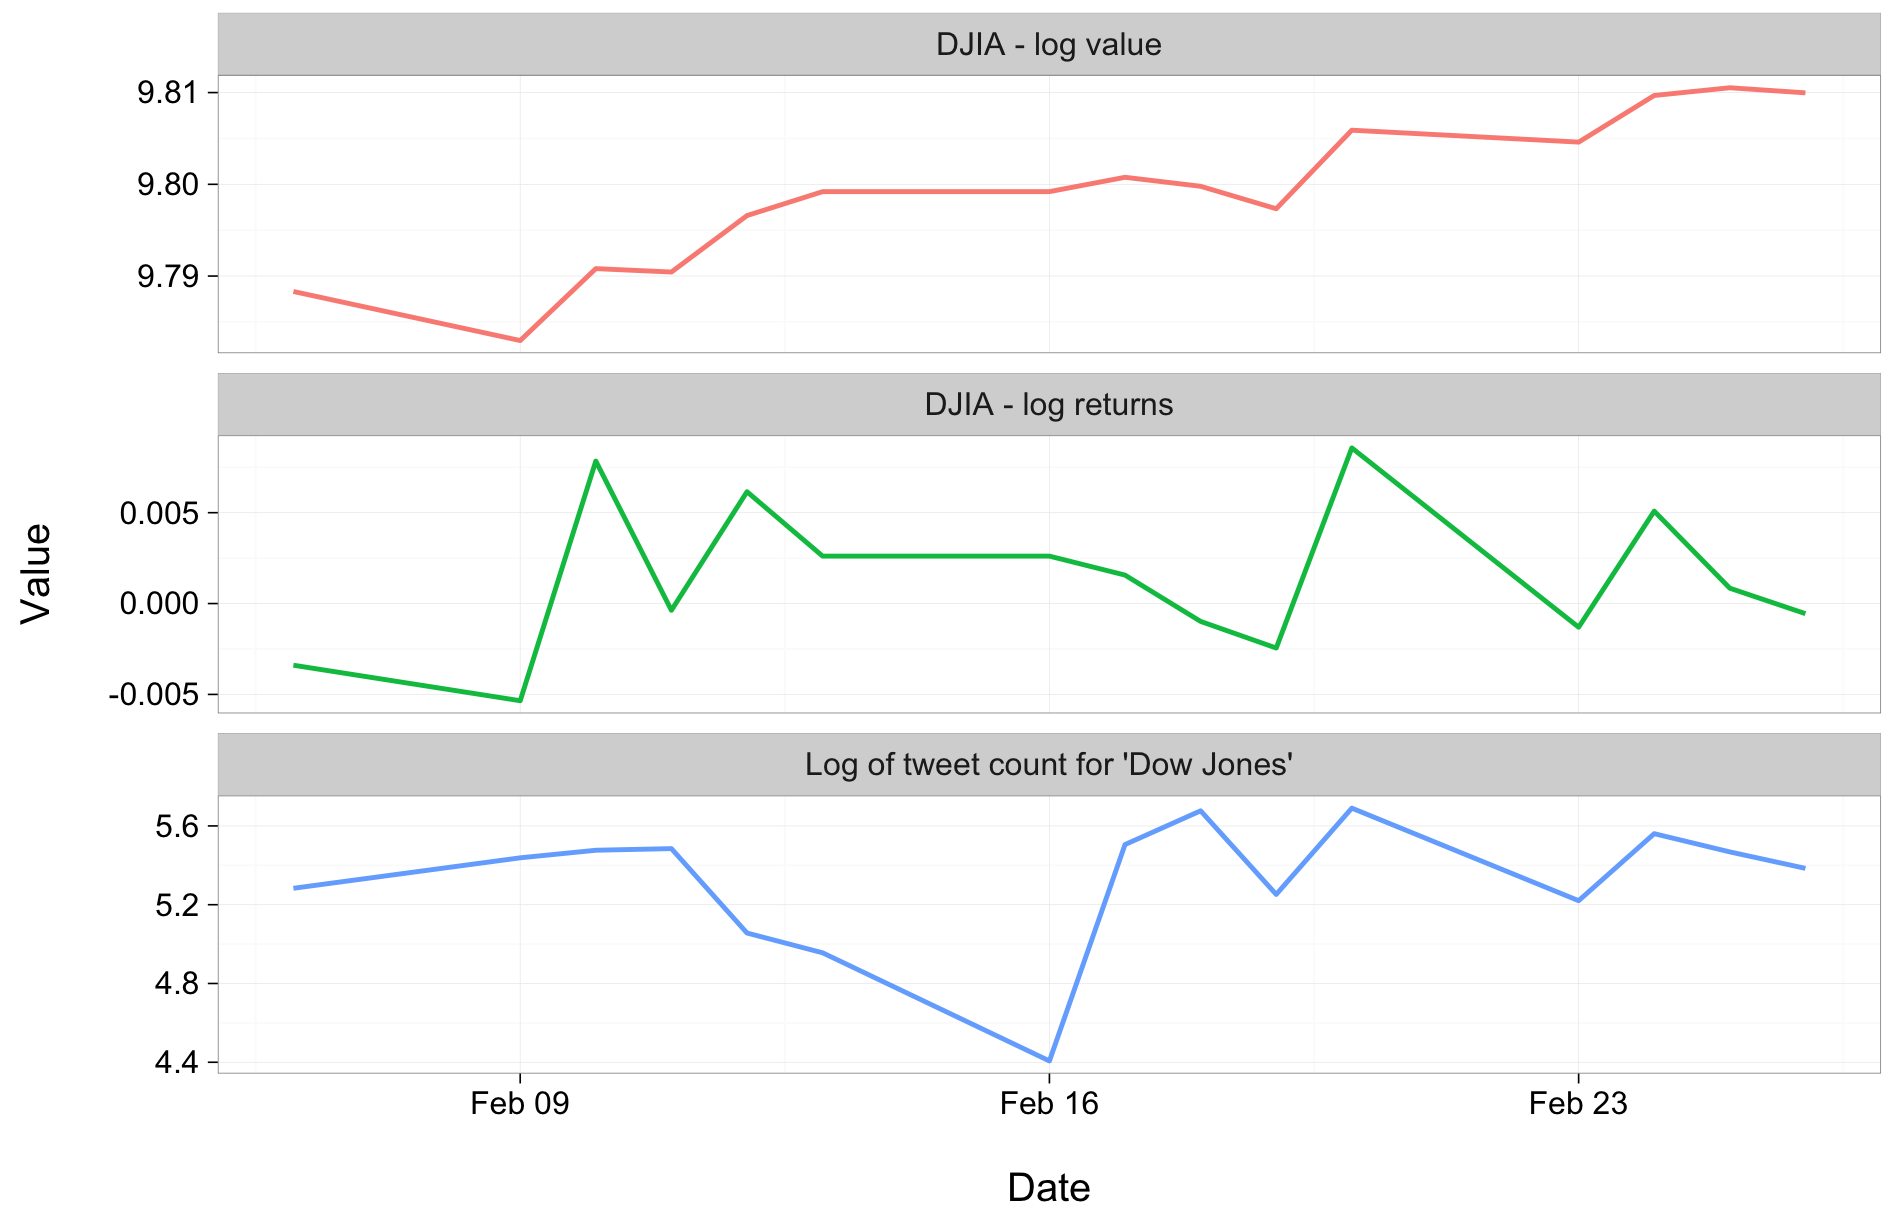
\includegraphics[width=16cm]{/Volumes/Mac OS Drive/Thesis/Source Code/Reporting/nwm_Report/images/DJIA_returns_tweet_count_three_weeks.png}
\caption[DJIA log-returns plotted alongside the logarithm of tweet counts]{\label{fig:day-to-day}Daily movements from 2015 in the DJIA - as well as the log returns thereof - are plotted against the log of sentiment scores for the same period from the "Dow Jones" search term.}
\end{figure}

\pagebreak


\subsection{Generalised linear models \label{main-modelling}}
\label{sec-1-4}

In this section, both a discussion of model parameters as well as results of the two main generalised linear models (GLMs) are presented, followed by a short comparison. Comparisons between the two GLM models, using component-wise boosting, and several differing models are provided in Section \texttt{results-summary}.


\subsubsection{Parameter grid \label{param-grid}}
\label{sec-1-4-1}

Parameters specific to the individual boosting step of the modelling (using the \texttt{mboost} package) are the learning rate, $\nu$, and the maximum number of iterations, $m_{max}$. A wide range were tested, resulting in a learning rate of $\nu = 0.05$, coupled with a maximum number of iterations $m_{max} = 2000$, which together sufficed for the algorithm to converge on all data sets. These values were therefore used, consistently, through all modelling variations. Using the bootstrap cross-validation method, outlined in Section \texttt{mstop}, meant that the optimal number of iterations $m_{stop}$ could be determined in each individual case, tailoring the final model used for prediction to each data set\footnote{In many cases, these values of $\nu$ and $m_{stop}$ were unnecessarily high. The disadvantage of this being computational cost, whereas the risk that was being circumnavigated was that of non-convergence. The latter is not a problem that cross-validation could have solved.}.

Taking a step back from each gradient descent problem, the next level of abstraction for the models in general concerns the \emph{time-series} nature of the data. It is desirable to make as many predictions as possible, allowing for the predictive accuracy and its errors to be computed accurately. For this reason, a final parameter was defined, namely the \emph{frame-size}, which describes how many days were used to approximate the optimal function $f^*$, using the pre-defined model parameters $\nu$ and $m_{stop}$ - the approximation function was then used to make one single prediction. As an example, using a frame-size equal to 40 means 40 periods of data were taken (40 days from the total 695), the boosting method generated the approximation function, which was subsequently used to predict the outcome variable on the 41$^{\text{st}}$ day.

One further modelling decision had to be made, namely whether the frame-size should be held constant (shifting along the timeline, one period at a time, with each shift making one prediction), or whether the start point be anchored, thereby allowing the number of periods used in finding the approximation function to grow over the timeline. When conducting time-series analysis, there are no hard-and-fast rules governing how many time-periods must be included to guarantee model robustness\footnote{As illustrated in the case of ARIMA modelling by \href{http://robjhyndman.com/hyndsight/short-time-series/}{R. Hyndman$^{\dag{}}$.}}. It is a question whose answer changes depending on the data being used. There is a trade-off to be found between three main components: the number of periods available, the number of covariates used (i.e. the number of model parameters to be estimated) and lastly the level of noise within the data set.

There are additional factors that must be taken into consideration within the context of financial markets, and those are of trends and cycles - not to be confused with seasonal effects, tackled through time-series decomposition. There are times in which an asset (e.g. a single company stock, a commodity or an entire index) tends to move in one direction, i.e. it exhibits some level of momentum. The event of such a cycle changing may be labelled a \emph{fraction} or \emph{break} in the asset's price-path\footnote{For work on modelling assets in such a fashion, refer to Mandelbrot's Multifractal Model of Asset Returns (MMAR) \cite{mandelbrot1997multifractal} \cite{calvet1997large} \cite{fisher1997multifractality}.}. The approach taken here to deal with this facet of financial time-series is to make use of our final parameter, frame-size, which would ideally be matched in length to those of the trends and cycles. This is difficult (perhaps impossible) to know ahead of time - and cannot be embedded into the model via the analysis of historic data\footnote{It is not possible using the data of this study. One can, however, envisage using older DJIA time-series data to estimate an optimal \emph{frame-size}.} without creating a bias in the predictions, as the information was not available at the time. Taking this into consideration, the choice was made to use a fixed frame-size for each model, shifting it along the timeline with each prediction. However, in order to test for ours model's sensitivity to the chosen frame-size, several values for this parameter were included in the parameter grid, namely 40 and 60 days.

In summary, the final set of parameters that were worked through included pair-combinations for the pairwise correlation threshold, $\kappa$, and the frame-size. For each of these pairs, every single subset (as defined in Section \ref{subsets}) was analysed and used to make predictions. The results are summarised in the following sections.   


\subsubsection{Gaussian family  \label{results-gauss}}
\label{sec-1-4-2}

The Gaussian family utilises the $L_2$ loss function (as depicted in Section \texttt{naive-boosting} by \eqref{eqn-gauss-loss} and \eqref{eqn-gauss-emp-risk}). Additional to several standard error measurements, we define a measurement, we shall call \emph{predictive accuracy}, which is a simple test that produces a binary response, indicating whether the \emph{direction} of movement was predicted correctly or not - the numerical discrepancy between the true and predicted values are not taken into consideration for this measure. In Figure \ref{fig:glm-pred-acc}, the column \emph{Predictive acc.} reports the percentage of correct predictions measured by the sign accuracy, over the ($695 -$ \emph{frame-size}) predictions that were made for each model.
Looking at the upper row of facet plots, with the frame-size fixed at 40 days, the \emph{combined} subset generally has the best performance, consistently appearing at the higher end of the predictive accuracy spectrum. The condensed \emph{sentiment$_{\text{small}}$} subset performed particularly well in cases with a lag of 1. As did the \emph{traditional$_{\text{small}}$} subset; however, that subset's performance decreased rather drastically with the increase of lag value, for all levels of $\kappa$.
With frame-size set to 60 in the lower row of plots, it is the \emph{sentiment$_{\text{large}}$} subset that dominates the group, producing some of the highest predictive accuracies, approaching 57 \%. The \emph{combined} subset performs similarly for lag values $\geqslant 2$. 

\begin{figure}[htb]
\centering
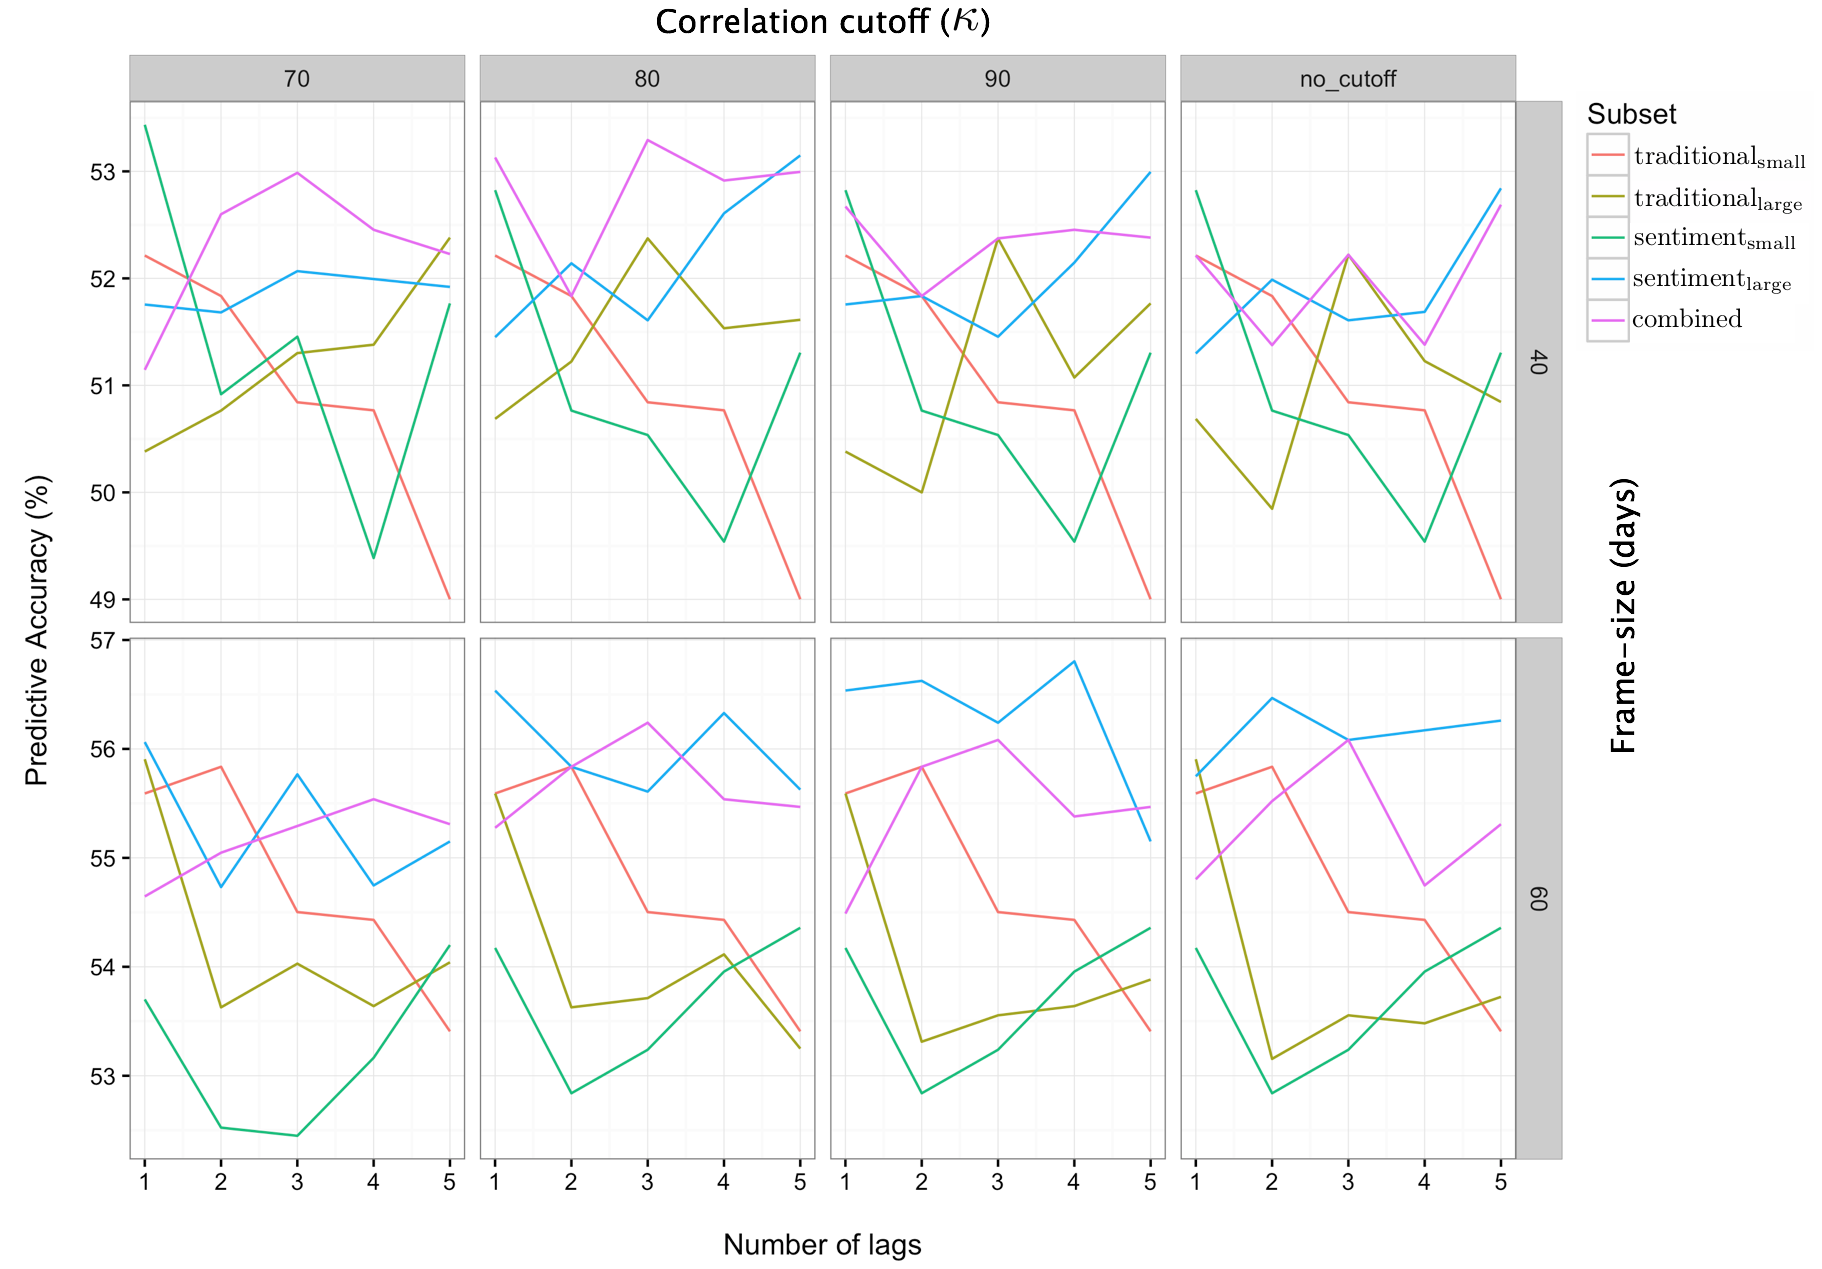
\includegraphics[width=16cm]{/Volumes/Mac OS Drive/Thesis/Source Code/Reporting/nwm_Report/images/glm_best_preds.png}
\caption[The predictive accuracy of all subsets, using Gaussian regression in GLMs]{\label{fig:glm-pred-acc}For each of the parameter-pairs, correlation cutoff $\kappa$ and frame-size (upper row 40 days, lower row 60 days), the average predictive accuracy is plotted for each subset, for each of its five lagged variants.}
\end{figure}

In Figure \ref{fig:glm-errors}, the mean-squared error (MSE) is given for each of the predictive accuracies presented in Figure \ref{fig:glm-pred-acc}. Each MSE value (just as with the predictive accuracy values) is the average value over the ($695 -$ \emph{frame-size}) predictions that were made for each subset. Comparing the upper and lower rows of plots, the errors are further spread out from one another within the upper row, with frame-size 40. In the facets where $\kappa$ = 70 \% and 80 \% (the two left-most columns), the errors of the \emph{combined} subset are at least as good as for all other subsets, with low dispersion between lags and low absolute values - they are very comparable to those of the $traditional_small$ subset. However, comparing the predictive accuracy of the two subsets in Figure \ref{fig:glm-pred-acc}, it can be seen that the \emph{combined} subset outperforms the \emph{traditional$_{\text{small}}$} subset in all but the first lag. In the plots where $\kappa$ = 90 \% and no correlation reduction was used (the two columns furthest to the right), there is a clear increase in error for both the \emph{sentiment$_{\text{large}}$} and \emph{combined} data sets. This is likely due to them containing a large number of predictors, which compounds as higher orders of lag are utilised (see Section \ref{subsets} for the number of predictors each subset contains). It appears to be in the first lag, where the two subsets are penalised most heavily for their size, relative to the other subsets. 

The errors of the \emph{sentiment$_{\text{small}}$} subset in the upper row, with a lag of 3, are noticeably larger than all others. A reason for the relatively high error value is unknown; however, the \emph{consistency} of the error (all values seemingly identical) may be explained by the fact that very few predictors are removed from this subset during the correlation reduction step described in Section \ref{pairwise-corr} - not unexpected, given the small number of predictors it begins with.

\begin{figure}[htb]
\centering
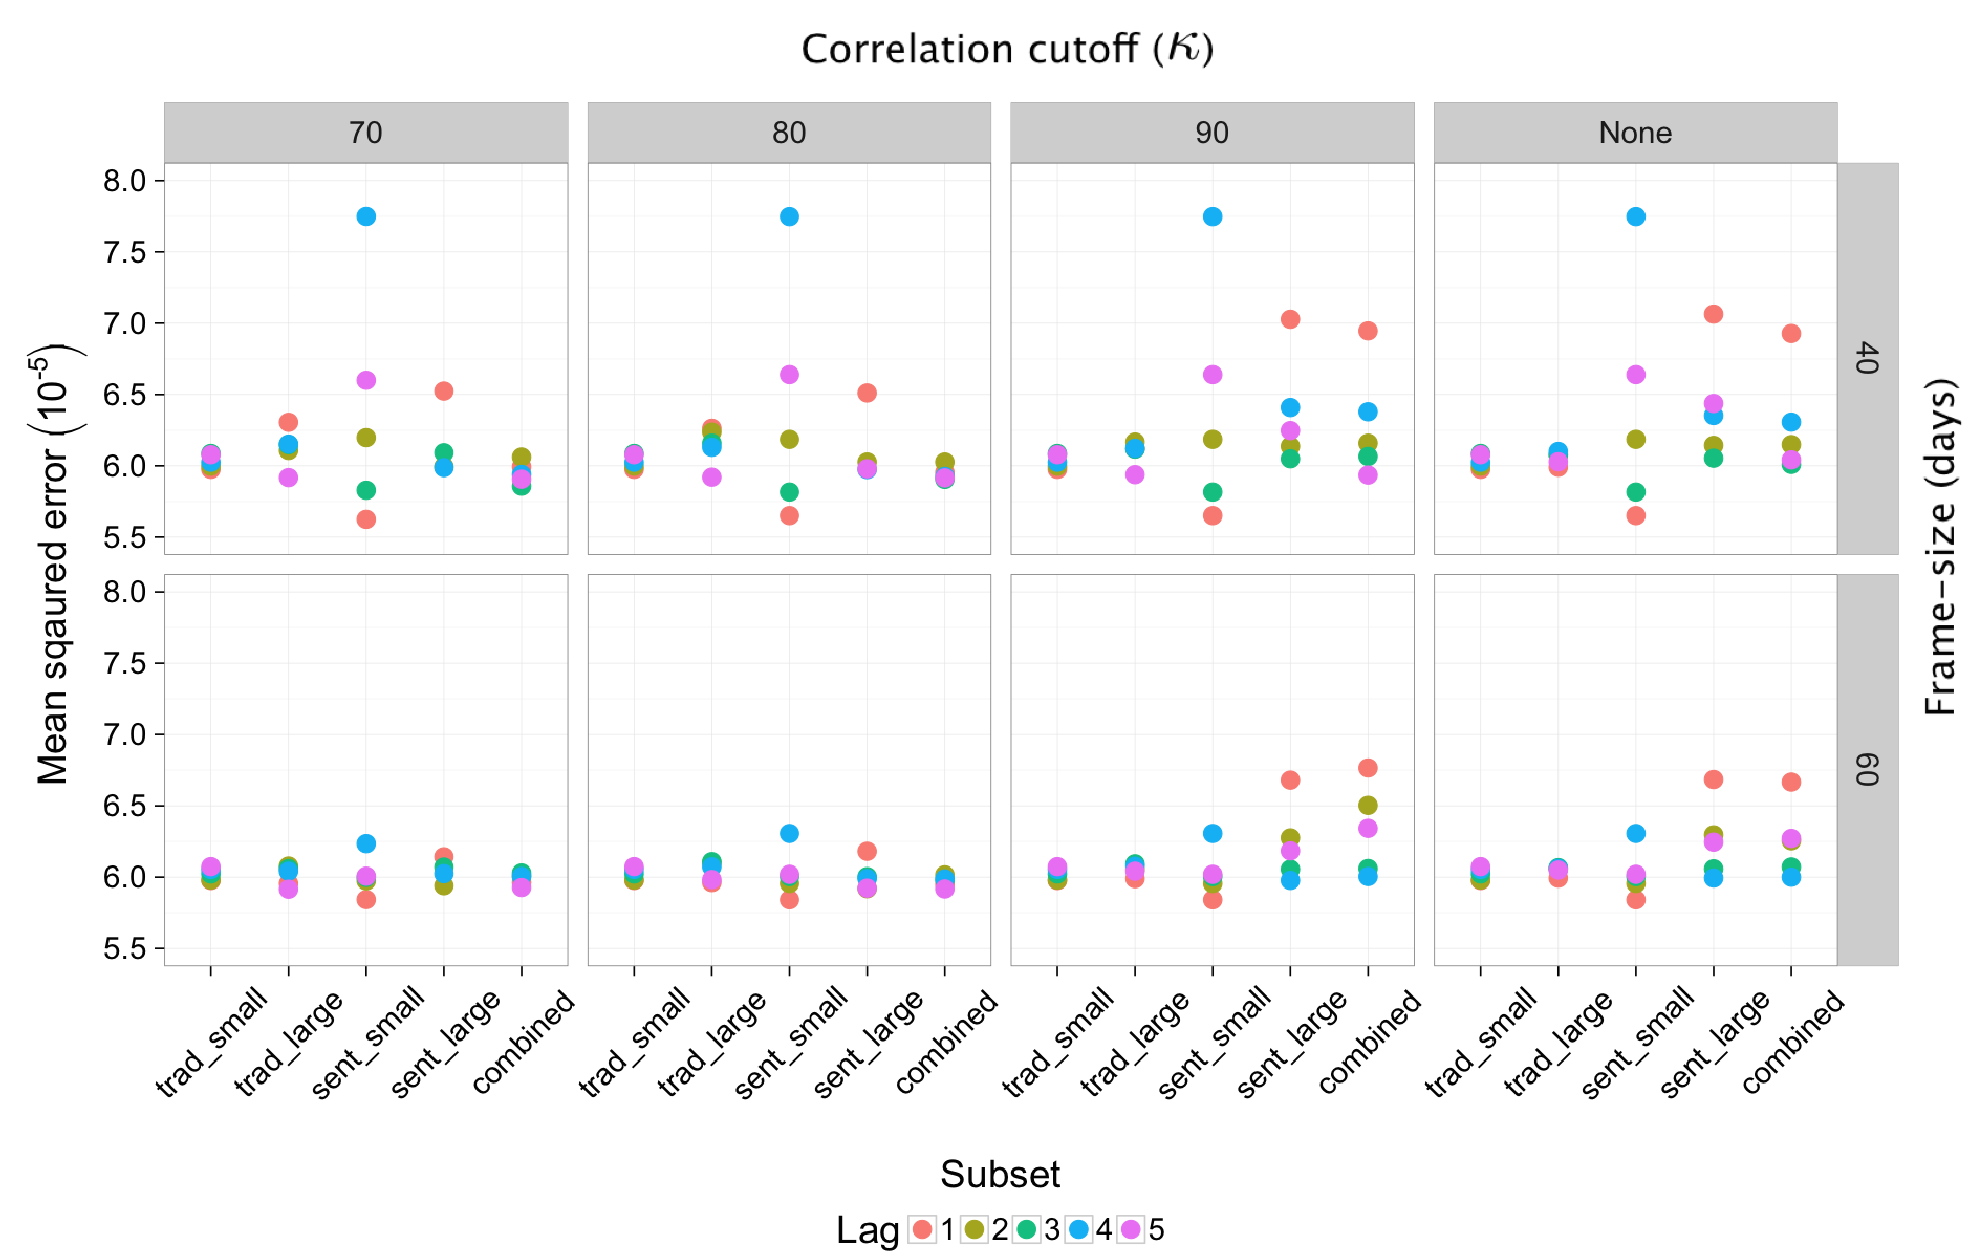
\includegraphics[width=16cm]{/Volumes/Mac OS Drive/Thesis/Source Code/Reporting/nwm_Report/images/glm_MSE_errors.png}
\caption[The mean-suared error of all subsets, using Gaussian regression in GLMs]{\label{fig:glm-errors}The mean-squared error for each of the results presented in Figure \ref{fig:glm-pred-acc}. Facets separate the frame-size and the correlation threshold $\kappa$ (upper row: 40 days, lower row: 60 days). The errors for each lag value of each subset are grouped onto one vertical line.}
\end{figure}


\subsubsection{Binomial family  \label{results-bin}}
\label{sec-1-4-3}

Each of the models that were presented in the previous section were also completed using the binomial family within the \texttt{mboost} package. Using this family meant that the outcome variable automatically produced a binary response, $\{0, 1\}$, which corresponded to the model predicting whether the market moves upwards or downwards on the following day. This is somewhat of a simplification in comparison to the models using the Gaussian family, as the question of magnitude is no longer a concern. The goal, therefore, was to increase the defined metric on performance, i.e. the predictive accuracy, by slightly reducing the requirements of the model. When predicting a binomial response, the ways in which error can be recorded are naturally confined. Numerical residuals cannot be measured for each prediction, as in the previous section. The two methods will, therefore, later be compared solely via their predictive accuracies.

As was done for the Gaussian family results, all parameter combinations for the binomial family are presented in Figure \ref{fig:bin-pred-acc}. Inspecting the upper row, which corresponds to a frame size of 40 days, it is clear that the \emph{combined} data set returns the greatest predictive accuracy for the majority of parameters combinations. The performance levels of the two \emph{small} data sets are equally low, barely breaching 51.5 \% predictive accuracy between them. The \emph{traditional$_{\text{large}}$} data set performs overall best in case where the lag was equal to five.

The lower row tells a more convincing story, with clear separation between the data sets that include sentiment analysis results and those that don't. The \emph{combined} and \emph{sentiment$_{\text{large}}$} subsets are clear victors across all values of $\kappa$ and lag; the \emph{sentiment$_{\text{small}}$} data  as performing markedly better than the two \emph{traditional} data sets. The \emph{combined} data set shows the highest predictive ability overall, with the \emph{sentiment$_{\text{large}}$} data set performing equally well when a larger frame-size was used. 

The models using a frame size of 60 days consistently outperform those using 40 days, with a relatively large improvement in predictive accuracy for almost every subset. The maximum predictive accuracy achieved in the latter equals that of the the worst in the former ($\approx$ 53 \%). These results validate the relationship pointed out in Section \ref{macro-view}, namely that long-term market momentum having ties with activity in social media. The inclusion of social media data, in this case, unquestionably improved the performance of the model.

\begin{figure}[htb]
\centering
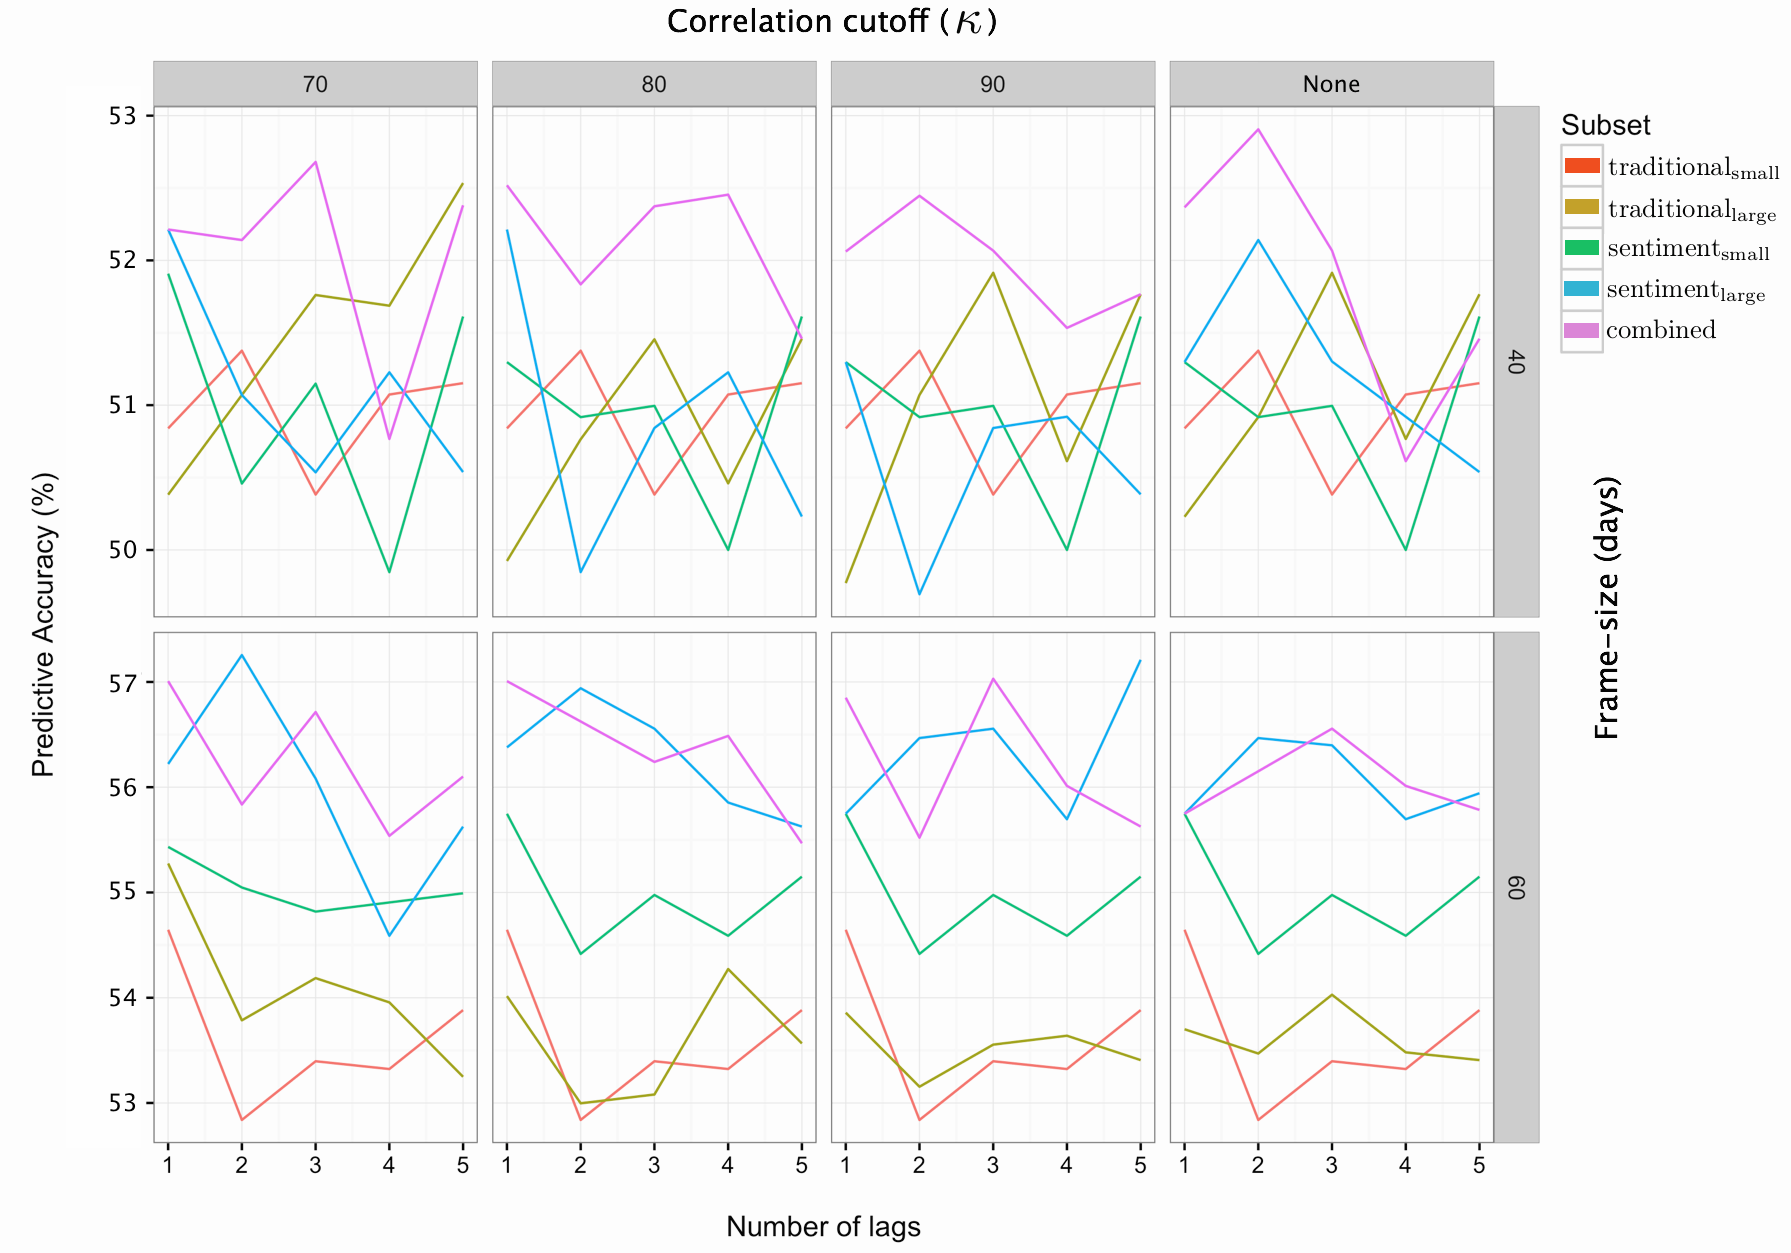
\includegraphics[width=16cm]{/Volumes/Mac OS Drive/Thesis/Source Code/Reporting/nwm_Report/images/bin_best_preds.png}
\caption[The predictive accuracy of all subsets, using binomial regression in GLMs]{\label{fig:bin-pred-acc}The predictive accuracies are plotted for the binomial model, separated by the frame-size and correlation threshold, $\kappa$ (upper row: 40 days, lower row: 60 days).}
\end{figure}

The top 50 results over all subsets and parameters combinations are given in Table \ref{tab:top-bin-results}, ordered according to predictive accuracy. The first \emph{traditional} subset appears at position 49. One thing that is highlighted by the results in that table is that the frame-size value of 60 dominates the results. This indicates that cycles of momentum in the DJIA (discussed briefly in Section \ref{param-grid}) appear to be best captured over a phase of 60 days\footnote{In the same table for the Gaussian results, the 60 day frame-size also dominates. The highest position a \emph{traditional} subset reached was 15$^{\text{th}}$; a total of 12 \emph{traditional} subsets appeared in the top 50.}. There is less consistency in the further parameters, $\kappa$ and lag. There is a general tendency for lower values of lag (1 to 3) to perform better.

\begin{table}\
\centering
\begin{tabular}{cclclclllc}
\textbf{Rank} & \textbf{Frame-size} &  & $\kappa$ \textbf{(\%)} &  & \textbf{Lag} &  & \textbf{Subset} &  & \textbf{Pred. accuracy (\%)}\\
 &  &  &  &  &  &  &  &  & \\
\hline
 &  &  &  &  &  &  &  &  & \\
1 & 60 &  & 70 &  & 2 &  & sentiment$_{\text{large}}$ &  & 57.26\\
2 & 60 &  & 90 &  & 5 &  & sentiment$_{\text{large}}$ &  & 57.21\\
3 & 60 &  & 90 &  & 3 &  & combined &  & 57.03\\
4 & 60 &  & 70 &  & 1 &  & combined &  & 57.01\\
5 & 60 &  & 80 &  & 1 &  & combined &  & 57.01\\
6 & 60 &  & 80 &  & 2 &  & sentiment$_{\text{large}}$ &  & 56.94\\
7 & 60 &  & 90 &  & 1 &  & combined &  & 56.85\\
8 & 60 &  & 70 &  & 3 &  & combined &  & 56.71\\
9 & 60 &  & 80 &  & 2 &  & combined &  & 56.62\\
10 & 60 &  & 80 &  & 3 &  & sentiment$_{\text{large}}$ &  & 56.56\\
11 & 60 &  & 90 &  & 3 &  & sentiment$_{\text{large}}$ &  & 56.56\\
12 & 60 &  & none &  & 3 &  & combined &  & 56.56\\
13 & 60 &  & 80 &  & 4 &  & combined &  & 56.49\\
14 & 60 &  & 90 &  & 2 &  & sentiment$_{\text{large}}$ &  & 56.47\\
15 & 60 &  & none &  & 2 &  & sentiment$_{\text{large}}$ &  & 56.47\\
16 & 60 &  & none &  & 3 &  & sentiment$_{\text{large}}$ &  & 56.40\\
17 & 60 &  & 80 &  & 1 &  & sentiment$_{\text{large}}$ &  & 56.38\\
18 & 60 &  & 80 &  & 3 &  & combined &  & 56.24\\
19 & 60 &  & 70 &  & 1 &  & sentiment$_{\text{large}}$ &  & 56.22\\
20 & 60 &  & none &  & 2 &  & combined &  & 56.15\\
21 & 60 &  & 70 &  & 5 &  & combined &  & 56.10\\
22 & 60 &  & 70 &  & 3 &  & sentiment$_{\text{large}}$ &  & 56.08\\
23 & 60 &  & 90 &  & 4 &  & combined &  & 56.01\\
24 & 60 &  & none &  & 4 &  & combined &  & 56.01\\
25 & 60 &  & none &  & 5 &  & sentiment$_{\text{large}}$ &  & 55.94\\
26 & 60 &  & 80 &  & 4 &  & sentiment$_{\text{large}}$ &  & 55.85\\
27 & 60 &  & 70 &  & 2 &  & combined &  & 55.84\\
28 & 60 &  & none &  & 5 &  & combined &  & 55.78\\
29 & 60 &  & 80 &  & 1 &  & sentiment$_{\text{small}}$ &  & 55.75\\
30 & 60 &  & 90 &  & 1 &  & sentiment$_{\text{small}}$ &  & 55.75\\
31 & 60 &  & 90 &  & 1 &  & sentiment$_{\text{large}}$ &  & 55.75\\
32 & 60 &  & none &  & 1 &  & sentiment$_{\text{small}}$ &  & 55.75\\
33 & 60 &  & none &  & 1 &  & sentiment$_{\text{large}}$ &  & 55.75\\
34 & 60 &  & none &  & 1 &  & combined &  & 55.75\\
35 & 60 &  & 90 &  & 4 &  & sentiment$_{\text{large}}$ &  & 55.70\\
36 & 60 &  & none &  & 4 &  & sentiment$_{\text{large}}$ &  & 55.70\\
37 & 40 &  & 80 &  & 3 &  & sentiment$_{\text{small}}$ &  & 55.65\\
38 & 40 &  & 90 &  & 3 &  & sentiment$_{\text{small}}$ &  & 55.65\\
39 & 40 &  & none &  & 3 &  & sentiment$_{\text{small}}$ &  & 55.65\\
40 & 60 &  & 70 &  & 5 &  & sentiment$_{\text{large}}$ &  & 55.63\\
41 & 60 &  & 80 &  & 5 &  & sentiment$_{\text{large}}$ &  & 55.63\\
42 & 60 &  & 90 &  & 5 &  & combined &  & 55.63\\
43 & 60 &  & 70 &  & 4 &  & combined &  & 55.54\\
44 & 60 &  & 90 &  & 2 &  & combined &  & 55.52\\
45 & 60 &  & 80 &  & 5 &  & combined &  & 55.47\\
46 & 60 &  & 70 &  & 1 &  & sentiment$_{\text{small}}$ &  & 55.43\\
47 & 40 &  & 70 &  & 3 &  & sentiment$_{\text{small}}$ &  & 55.31\\
48 & 40 &  & 90 &  & 1 &  & sentiment$_{\text{large}}$ &  & 55.29\\
49 & 60 &  & 70 &  & 1 &  & traditional$_{\text{large}}$ &  & 55.28\\
50 & 40 &  & 80 &  & 4 &  & sentiment$_{\text{small}}$ &  & 55.24\\
\end{tabular}\caption[The top 50 binomial models, ranked by descending predictive accuracy]{\label{tab:top-bin-results}The top 50 predictive accuracies from the binomial models. The results are dominates by subsets containing sentiment analysis data. The best performing traditional model appears at position 49.}

\end{table}

\pagebreak


\subsubsection{Family comparisons}
\label{sec-1-4-4}

Inspecting first the predictive accuracy results in Figures \ref{fig:glm-pred-acc} and \ref{fig:bin-pred-acc}, as well as the detailed results found in Table \ref{tab:top-bin-results} for the binomial results, we see that the best performers are unequivocally those containing social media and sentiment analysis data. The magnitude of the predictive accuracies are very similar between the Gaussian and binomial sets of results, ranging from 50 \% to 53 \% for frame sizes of 40, and from 53 \% to just over 57 \% in the case of a 60 day frame-size. The clear distinguishing feature between the two families is the separation of performance between models containing social media data and those that didn't, that the binomial family was able to accentuate. Other than this difference, the two models are not easy to distinguish between in terms of their performance. Due to the binomial model not returning MSE values, it is not possible to compare the errors of the two models.

Almost each model outperformed a naive (random selection) model giving 50\% predictive accuracy. Only in the cases of the small data sets; \emph{traditional$_{\text{small}}$} and \emph{sentiment$_{\text{small}}$} in lag values four and five, with a frame size of 40 days, were any results worse than 50 \% found.


\subsubsection{Prediction-generated price paths \label{price-paths}}
\label{sec-1-4-5}

Figure \ref{fig:price-paths} visualises the results in direct comparison to the DJIA itself, by plotting its price-path over the entire timeline against those price-paths that were predicted (on a day-by-day basis) by several different models. In order to have measurable magnitudes of price movement, the results from the Gaussian GLM models are used. The prices follow from a nominal base-value of 100. We take the \emph{combined} data set that performed the best over all parameters configurations, namely for: frame-size $= 60$, $\kappa$ = 80 \% , with a lag of 3. In comparison, we take the \emph{traditional$_{\text{large}}$} data set (thereby containing all the same financial market data, but without the social media data) for the same parameter combinations, plus a third data set, which is the best performing \emph{traditional} subset. That used the parameters frame-size $= 60$, $\kappa$ = 70 \%, with a lag of 1.

\begin{figure}[htb]
\centering
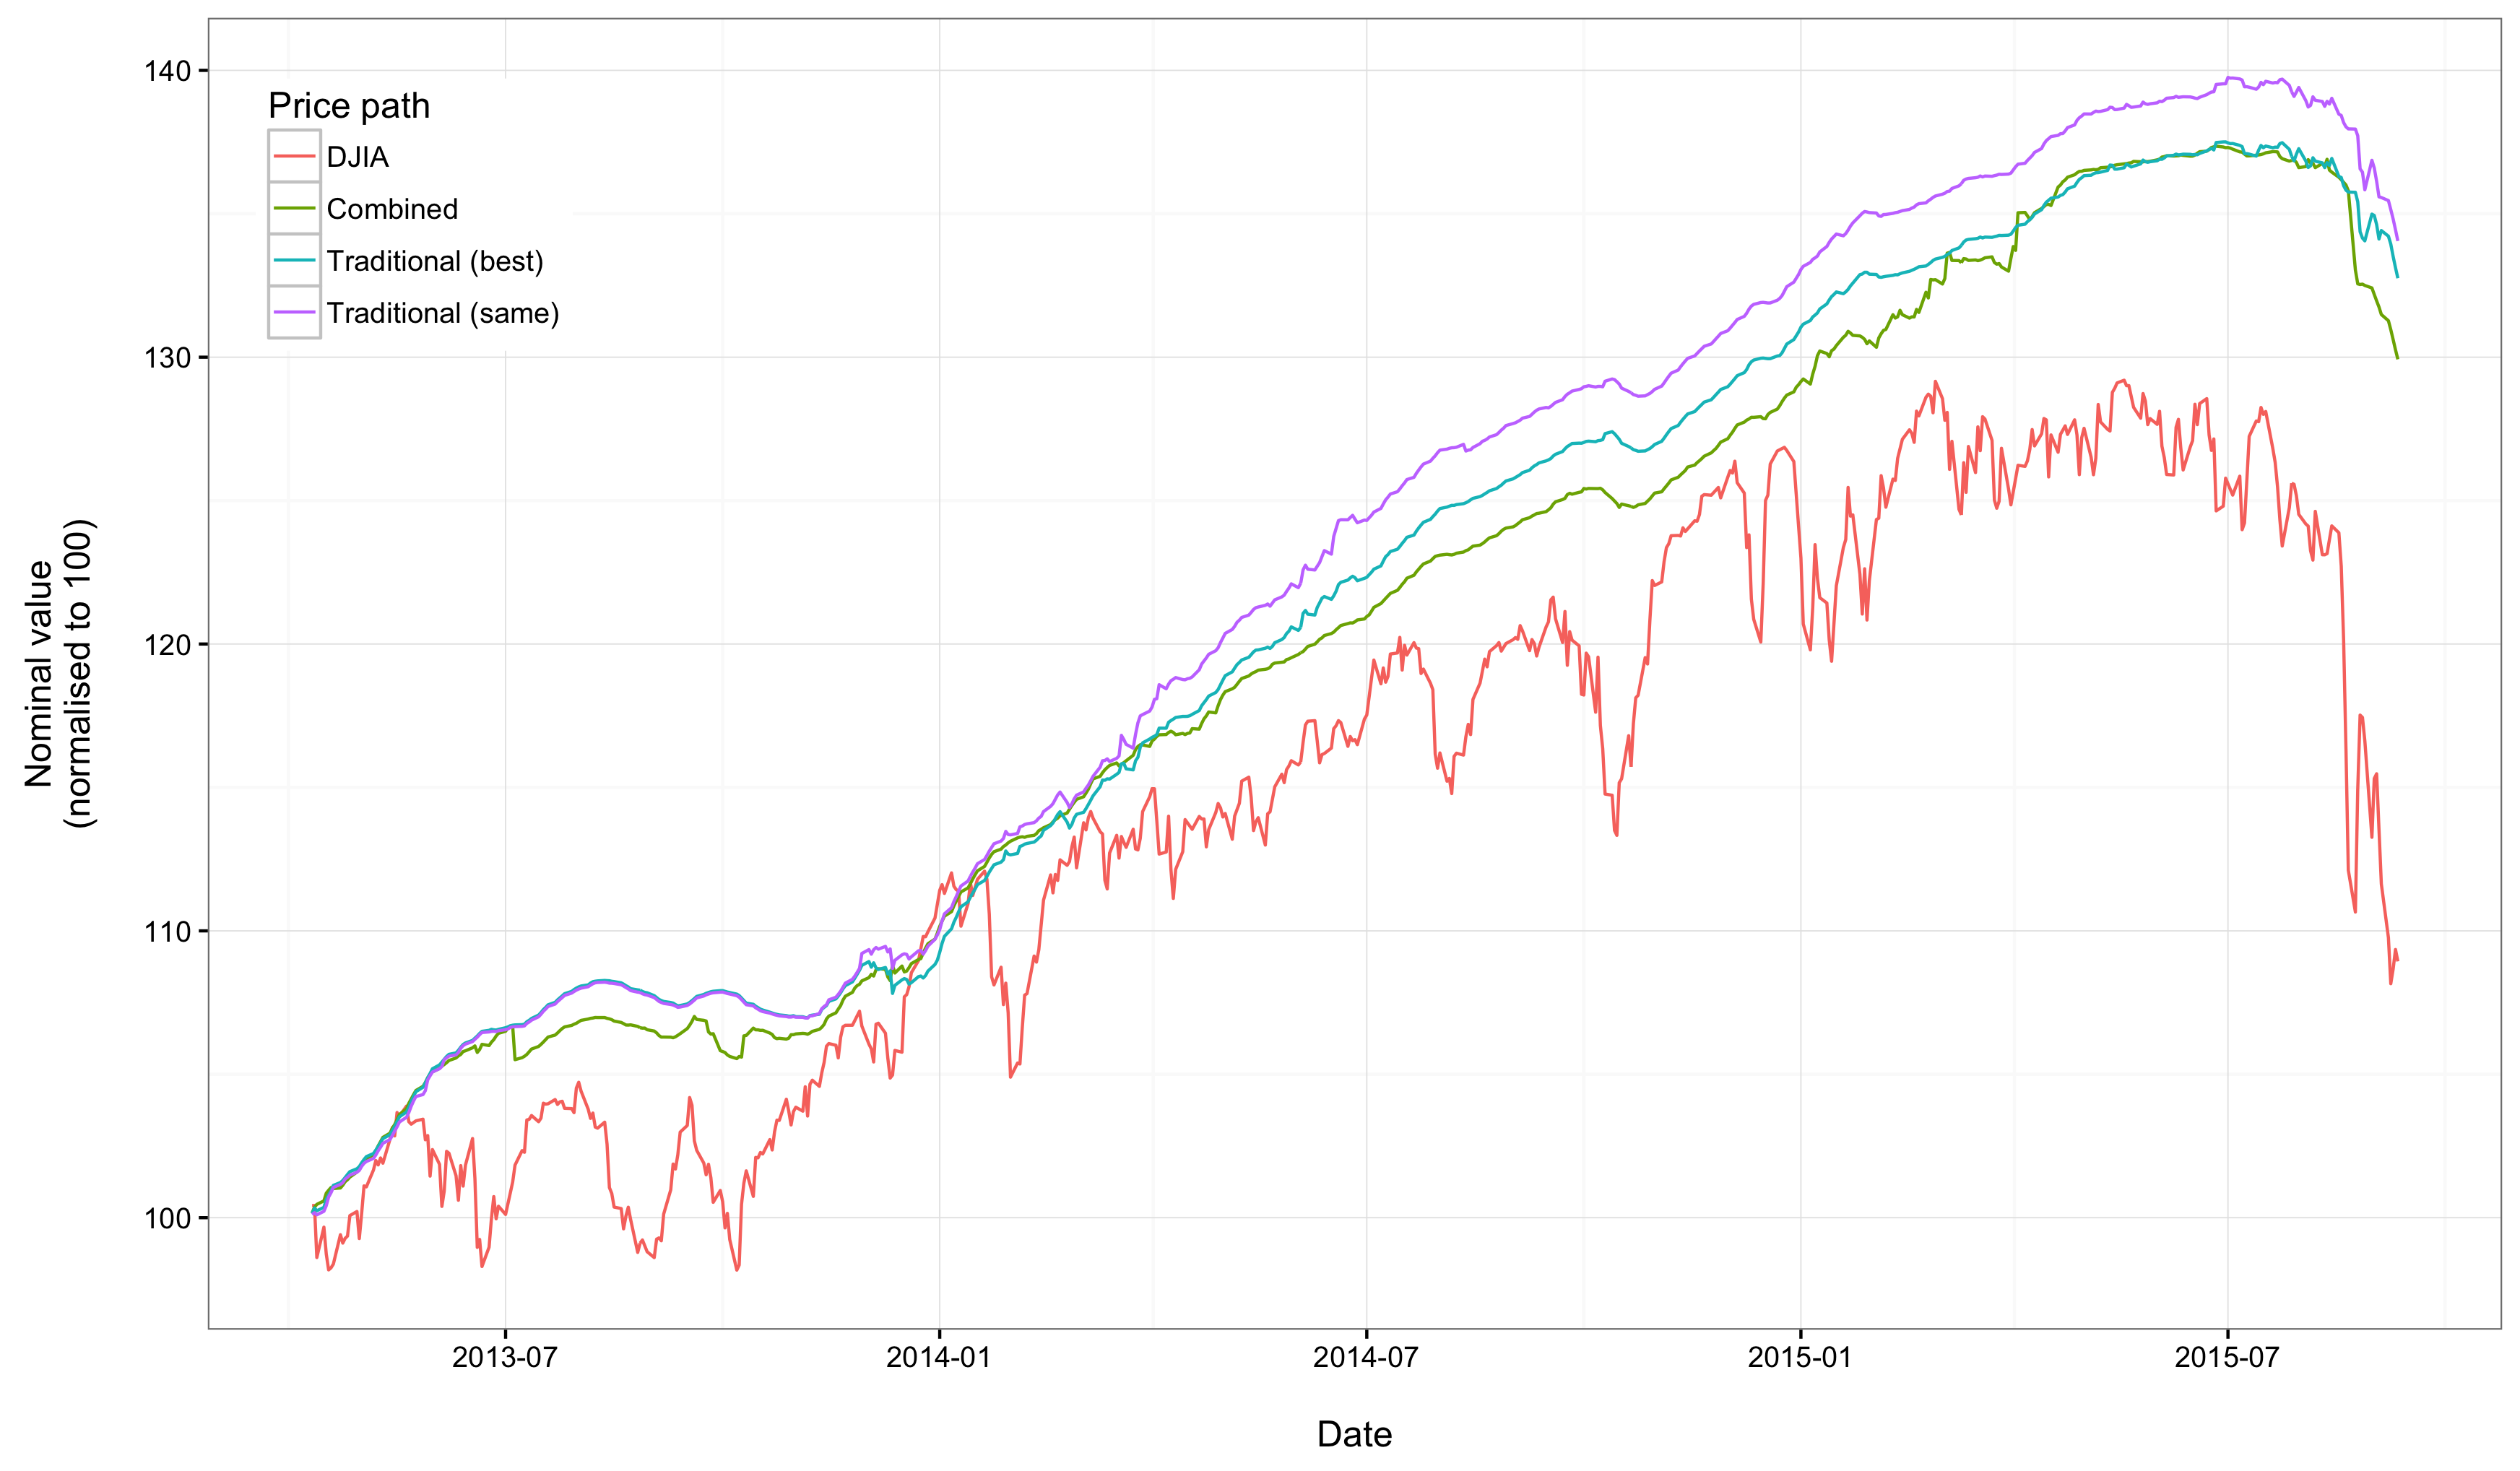
\includegraphics[width=16cm]{/Volumes/Mac OS Drive/Thesis/Source Code/Reporting/nwm_Report/images/price_paths.png}
\caption[Four price-paths, comparing forecasted returns against actual returns]{\label{fig:price-paths}Four price-paths are plotted over the entire timeline: the DJIA plus those of the three best performing \emph{combined} and \emph{traditional} data sets, as described in Section \ref{price-paths}.}
\end{figure}

All three of the predicted returns manage to map to the movements of the market fairly well - following similar patterns of peaks and troughs. It is the \emph{combined} data set that most closely resembles the price-path of the the DJIA, more intimately tracking movements and reacting more sharply to large jumps the DJIA made. For example, all three subsets move as expected on the news of the huge drop on 24$^{\text{th}}$ August 2015 (discussed in Section \ref{macro-view}); however, it is the \emph{combined} data set, including social media data, which falls earliest and most rapidly, thereby most closely reflecting the DJIA. All three of the subsets produce paths that somewhat resemble a moving average of the DJIA itself, all with an upward bias and without the high levels of granularity exhibited by the DJIA.


\subsubsection{Increasing frame-size}
\label{sec-1-4-6}

Throughout the modelling presented thus far, the frame-size used to train an approximation function was fixed at either 40 or 60 days. The reasons for which are discussed in Section \ref{param-grid}. Here we present a set of predictive accuracy results that were created - for the Gaussian and binomial models - using an \emph{increasing} frame-size. An initial frame-site of 60 days was used; however, instead of shifting the frame along one day into the future to train a new approximation function and, from that, make one more prediction, the frame-size was increased by one day and \textbf{not shifted} - keeping the start of the frame-size anchored at day 1 in the timeline. This means that, for each prediction, the maximum amount of information available within the data set was used, i.e. all days in the timeline up until the day before the prediction. This is to test the assumption that the frame-size corresponds to general trends and phases within the price development of the DJIA. The approach presented here has the advantage that the maximum possible amount of information is used for every prediction (in terms of the timeline), but has perhaps a disadvantage in that it does not necessarily capture the prevailing momentum of the market at the time of the prediction.

In addition to an (initial) frame-size of 60 days being used (as with all other comparisons made to the results from Section \ref{main-modelling}), a correlation threshold of $\kappa$ = 80 \% was used. All other model parameters, such as shrinkage, $\nu = 0.05$, and maximum number of boosting iterations, $m_{max} = 2000$, were kept identical to those used in Section \ref{main-modelling}, for both the Gaussian and binomial models. Figure \ref{fig:growing-frame} presents the predictive accuracies of the two comparisons, with the left column displaying the results of the binomial model and the right column those of the Gaussian model. In both columns, the upper row gives the results obtained earlier from a fixed frame-size of 60 days, whilst the lower row gives those for an increasing frame-size. 

\vspace{3mm}

\begin{figure}[htb]
\centering
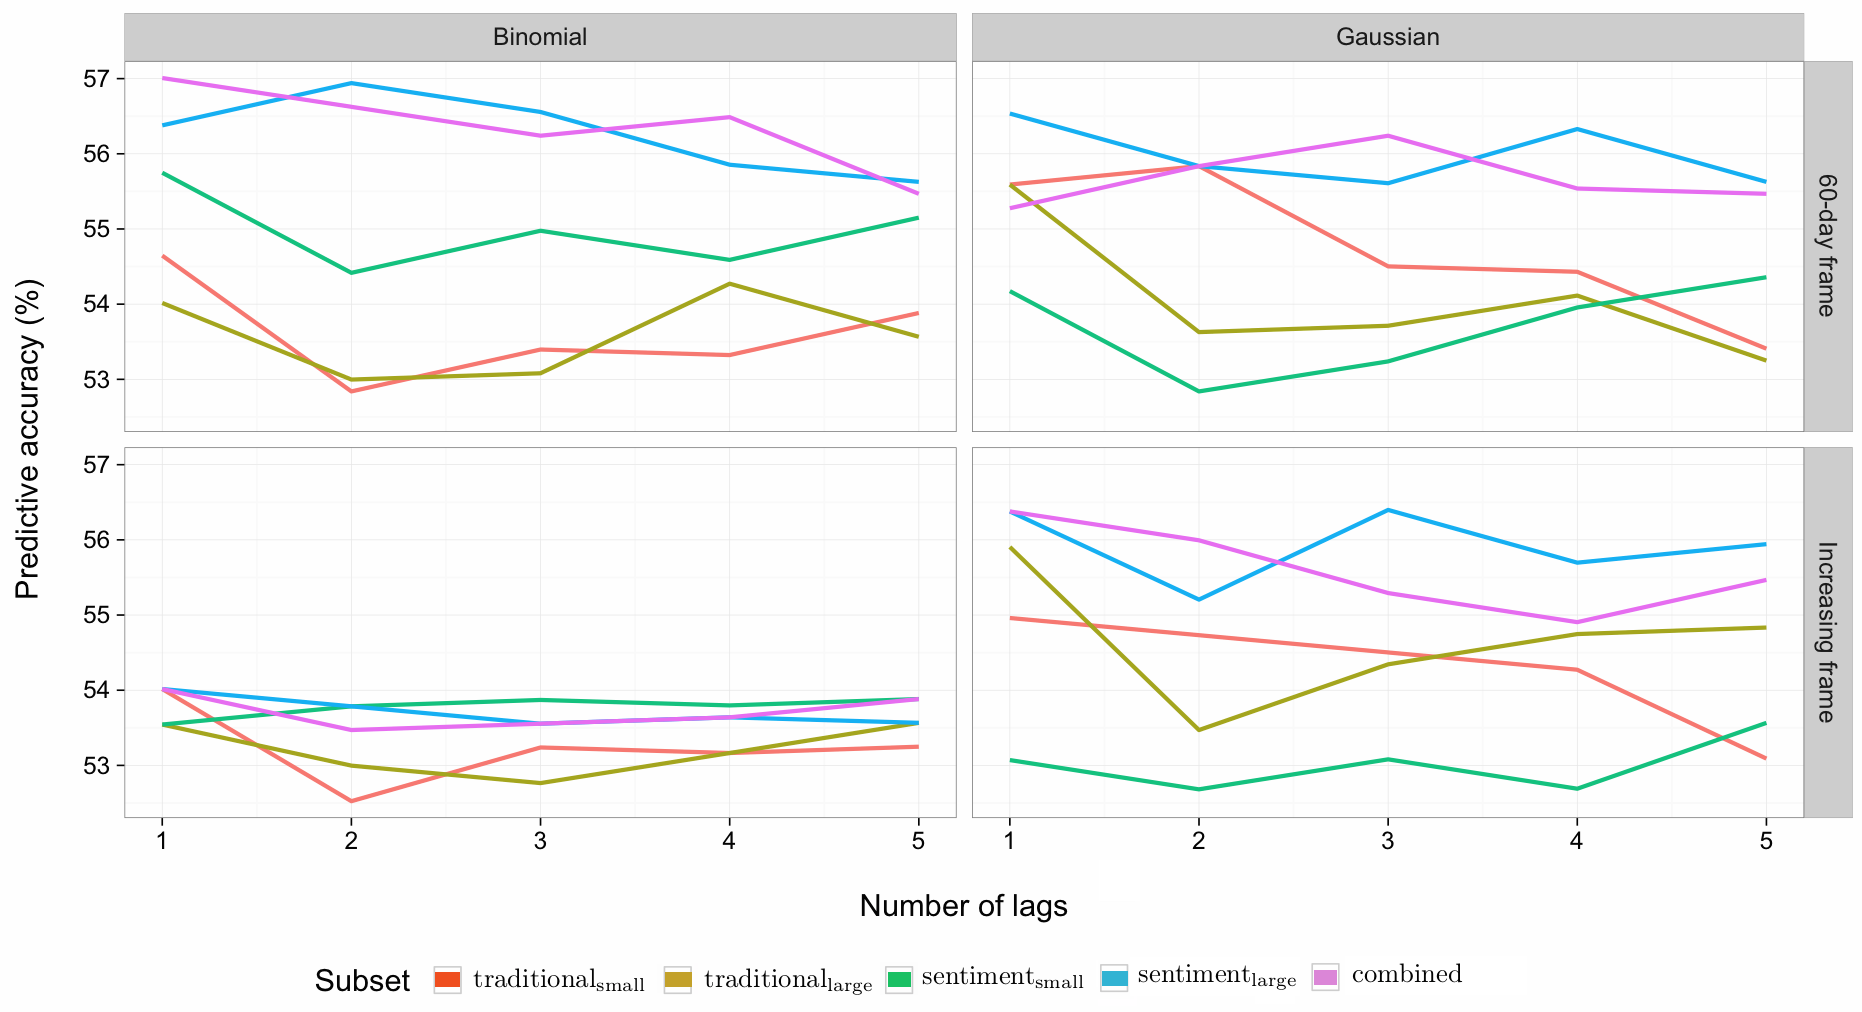
\includegraphics[width=16cm]{/Volumes/Mac OS Drive/Thesis/Source Code/Reporting/nwm_Report/images/growing_plain_frame.png}
\caption[The predictive accuracies of GLMs using fixed versus increasing frame-size]{\label{fig:growing-frame}A comparison of predictive accuracies between models with fixed frame-size and increasing frame-size. In both cases, results using binomial (left) and Gaussian (right) modelling are plotted. Each facet contains the results for all lagged variants of all five subsets.}
\end{figure}

Inspecting first the binomial results, it is evident that the use of an increasing frame-size significantly diminishes the performance of the model. All predictive accuracies are compressed to below 54 \%, with the \emph{traditional} subsets still showing weaker performance than those subsets containing social media data. While still performing worse than in the case of a fixed frame-size, the \emph{sentiment$_{\text{small}}$} subset did manage to surpass the other subsets in all but the first lagged variant, when using the increasing frame-size. This may be due to more information being provided (due to a higher average number of periods used for each prediction), while still being compactly included in fewer covariates than in the other models.

In the case of the Gaussian models, the performance is very similar between the models using fixed frame-size and those with increasing frame-size. The predictive accuracy of the \emph{combined} data set increases in the first lag, from 55.5 \% with fixed frame-size to 56.5 \% with increasing frame-size. It is indistinguishable in the second lag ($\approx$ 56 \%), while the performance is reduced for lags three, four and five. It is perhaps juxtapositional to state that the high number of variables, coupled with ever increasing numbers of observations overwhelms the boosting algorithm because, contradictorily, the performance of the \emph{sentiment$_{\text{large}}$} data set actually improves along the same dimension of comparison - it shows higher performance in lags three and five for the increasing frame-size method than that of fixed frame-size. The \emph{sentiment$_{\text{small}}$} data set performs consistently worse using an increasing frame-size that fixed, which may reflect the model losing its ability to explain market momentum when presented with longer time-frames, using only its succinct collection of predictors. Sentiment seems only to aid with prediction in the shorter term. This can also be seen when looking at the simulated price-paths illustrated in Section \ref{price-paths}, where the \emph{combined} data set was better attuned to market movements than its \emph{traditional$_{\text{large}}$} counterpart in the short-term.

Comparing the binomial and Gaussian models, it seems the Gaussian regression methods was better able to cope with the higher influx of data at each iteration, whereas the binomial model was more greatly, negatively, affected.



\subsection{Stochastic gradient boosting \label{stochastic-boosting}}
\label{sec-1-5}


\subsubsection{Parameter tuning}
\label{sec-1-5-1}

This section presents results obtained from stochastic gradient boosting, which was performed for a binary response variable, i.e. whether the market rose or fell. This makes for good comparison to the results presented in Section \ref{results-bin}, however the methodology does differ in more than one way. A detailed discussion on stochastic gradient boosting may be found in Section \ref{stochastic-boosting}. It must be made very clear that the algorithm used here is \textbf{not} component-wise gradient boosting, but rather the \emph{batch} gradient boosting, outlined in Section \texttt{naive-boosting}. As this stochastic methodology is quite different, the aim here is merely to achieve the best \emph{predictive accuracy} possible using the stochastic approach. Results are then be compared to those presented in Section \ref{results-bin} via this metric, which is validated by the choice of input data (see below). Using the \emph{batch} gradient descent method does raise concerns about performance in the face of wide data sets, as there is no in-built variable selection. We aim to test the abilities the method has through its added factor of random predictor selection, which essentially replaces that of the more systematic and statistically tuneable way of sequential variable selection, carried out in component-wise gradient boosting. The added randomisation does not compensate directly for this difference, however it is designed (adapted to utilise properties of random forests) to have the ability of variance reduction within a model (see section \ref{stochastic-boosting}).

In order to compare the performance of a stochastic implementation of gradient boosting as fairly as possible with that of the GLM models using component-wise boosting, an identical subset of this study's data set was used. Namely that with a correlation threshold, $\kappa$ = 80 \%, with lag values one through five. The methodology followed here does mean that the \emph{frame-size} parameter is lost. This is because, instead of using a rolling-window approach, train a test sets were created instead of sequentially fitting a model and making a prediction at one-period intervals along the timeline\footnote{This was also because the limitations of the R package \texttt{gbm}, which did not to be function when using the narrower of the data sets, e.g. \emph{traditional$_{\text{small}}$} and \emph{sentiment$_{\text{small}}$}.}. The 25 data sets - the five lags of each of the five subsets - were each divided into 65 \% training data and 35 \% test data, using stratified sampling. If it is assumed that the market rose and fell with a ratio of e.g. 8:10 over all periods, then \emph{stratified} sampling simply signifies that the training and test sets created also contain this ratio of days, on which the market rose and fell. A model was then trained on the training set (of 452 days) and the test set (243 days) was used to make predictions. The predictive accuracy was then defined as the percentage of days on which the movement of the market was correctly predicted, out of the 243 predictions made.

Using this method introduces several new paramters to the model, the most interesting of which being the fraction of predictors\footnote{In his original paper \cite{friedman2002stochastic}, Friedman used $\pi$ to symbolise a random permutation of the data, from which the fraction was taken. We use $\pi$ simply to symbolise the fraction, or sub-sample, of of predictors used to fit the base learner in a given step.} that are randomly selected at each iteration of the gradient descent process, $\pi$. This paramter generally leads to a slower descent of the loss function, meaning a larger number of iterations are required. Furthemore, it allows several other \emph{new} hyperparamters to be tuned. To optimise for these, a new parameter tuning grid was first defined to test over a wide range of combinations\footnote{As was mentioned, the frame-size no longer plays a role, and the value of $\kappa$ remained fixed at 80 \%.}. The metric used to tune the paramters was the area under the \href{https://en.wikipedia.org/wiki/Receiver_operating_characteristic}{receiver operator characteristic$^{\dag{}}$} (AUROC) \cite{bradley1997use}. This tuning was performed individually for each of the data sets, as their differences in size may have been better suited to different variations to the model parameter space. Table \ref{tab:tuning-grid} shows the values that were tested for, as well the the values for each parameter that were given as optimal in the case of the \emph{combined} data set with lag value of 5 - the largest data set. The optimal random selection fraction, $\pi$, was found to be 0.5, which coincides with the range suggestion made by Friedman \cite{friedmanstochastic}. The maxmimum number of boosting iterations, $m_{max}$ was given to be 3000, which is 50 \% more than was found to be a reasonable maximum for the component-wise boosting. Again, the number of iterations required to reached the loss-function's minimum is expected to increase, as the introduction of a stochastic process perturbs the path of steepest descent - the added benefit (as discussed in Section \ref{stochastic-boosting}) being that variance in results is likely reduced. An optimal learning rate of $\nu = 0.01$ further reflects that the algorithm is required to be a slow learner with the involvement of a stochastic process.

\vspace{5mm}

\begin{table}[htb]
\centering
\begin{tabular}{clllllc}
\textbf{Parameter} &  & \textbf{Value range} &  & \textbf{Desctiption} &  & \textbf{Optimum}\\
 &  &  &  &  &  & \\
\hline
 &  &  &  &  &  & \\
$\pi$ &  & 0.3, 0.5, 0.7 &  & The fraction of parameters &  & 0.5\\
 &  &  &  & selected at each iteration &  & \\
 &  &  &  &  &  & \\
$m_{max}$ &  & 100 - 5000 (intervals of 500) &  & The number of iterations &  & 3000\\
 &  &  &  &  &  & \\
$\nu$ &  & 0.01, 0.05, 0.1 &  & The learning rate, or shrinkage &  & 0.01\\
 &  &  &  &  &  & \\
\end{tabular}\caption[The tuning grid optimised over for stochastic gradient boosting]{\label{tab:tuning-grid}The tuning grid used to find optimal parameters for the stochastic gradient boosting algorithm, for binary response modelling.}

\end{table}


\subsubsection{Comparison to component-wise boosting}
\label{sec-1-5-2}

The results of the stochastic gradient boosting are compared to those of the GLM model using component-wise boosting, originally presented in Section \ref{results-bin}. As was mentioned there, the two methods are similar, but not the same. Therefore, any comparisons deeper than that of the pure outcome, the \emph{predictive accuracy}, are not possible within the scope of this limited superficial differentiation of their nuances.

It can be seen from Figure \ref{fig:stoch-pred-acc} that the results obtained from the stochastic boosting are not as strong as those from component-wise boosting, with several models failing to beat even a naive model with predictive accuracy of 50\%, with the performance of the \emph{traditional$_{\text{large}}$} subset dropping below 47.5 \% in one case (in lag 1). Furthermore, the stochastic boosting results do not show any signs of reduced variance\footnote{The reduction in variance through the addition of a stochastic process is usually detectable through lower errors (and variance thereof) on predictions; however, these are not available here, having performed logistic regression.}, when compared to the component-wise boosting results. The relatively large spread in performance within the stochastic boosting results is clear to see, with almost 10 \% difference between the best (\emph{sentiment$_{\text{small}}$} in lag 2) and worst (\emph{traditional$_{\text{large}}$} in lag 1) performers, which is larger than any other set of boosting results found in this study.

The ability of stochastic boosting to deal with the larger data sets seems to also be inferior to that of component-wise boosting. This is illustrated by the superior performance of the smaller data sets, with both the \emph{sentiment$_{\text{small}}$} and the \emph{traditional$_{\text{small}}$} subsets outperforming their \emph{large} equivalents in four out of five lag variants. The largest subset: \emph{combined}, performs unexpectedly poorly, given its comparatively high levels of predictive accuracy in all parameter combinations used in component-wise boosting, depicted in Sections \ref{results-gauss} and \ref{results-bin}.

\begin{figure}[htb]
\centering
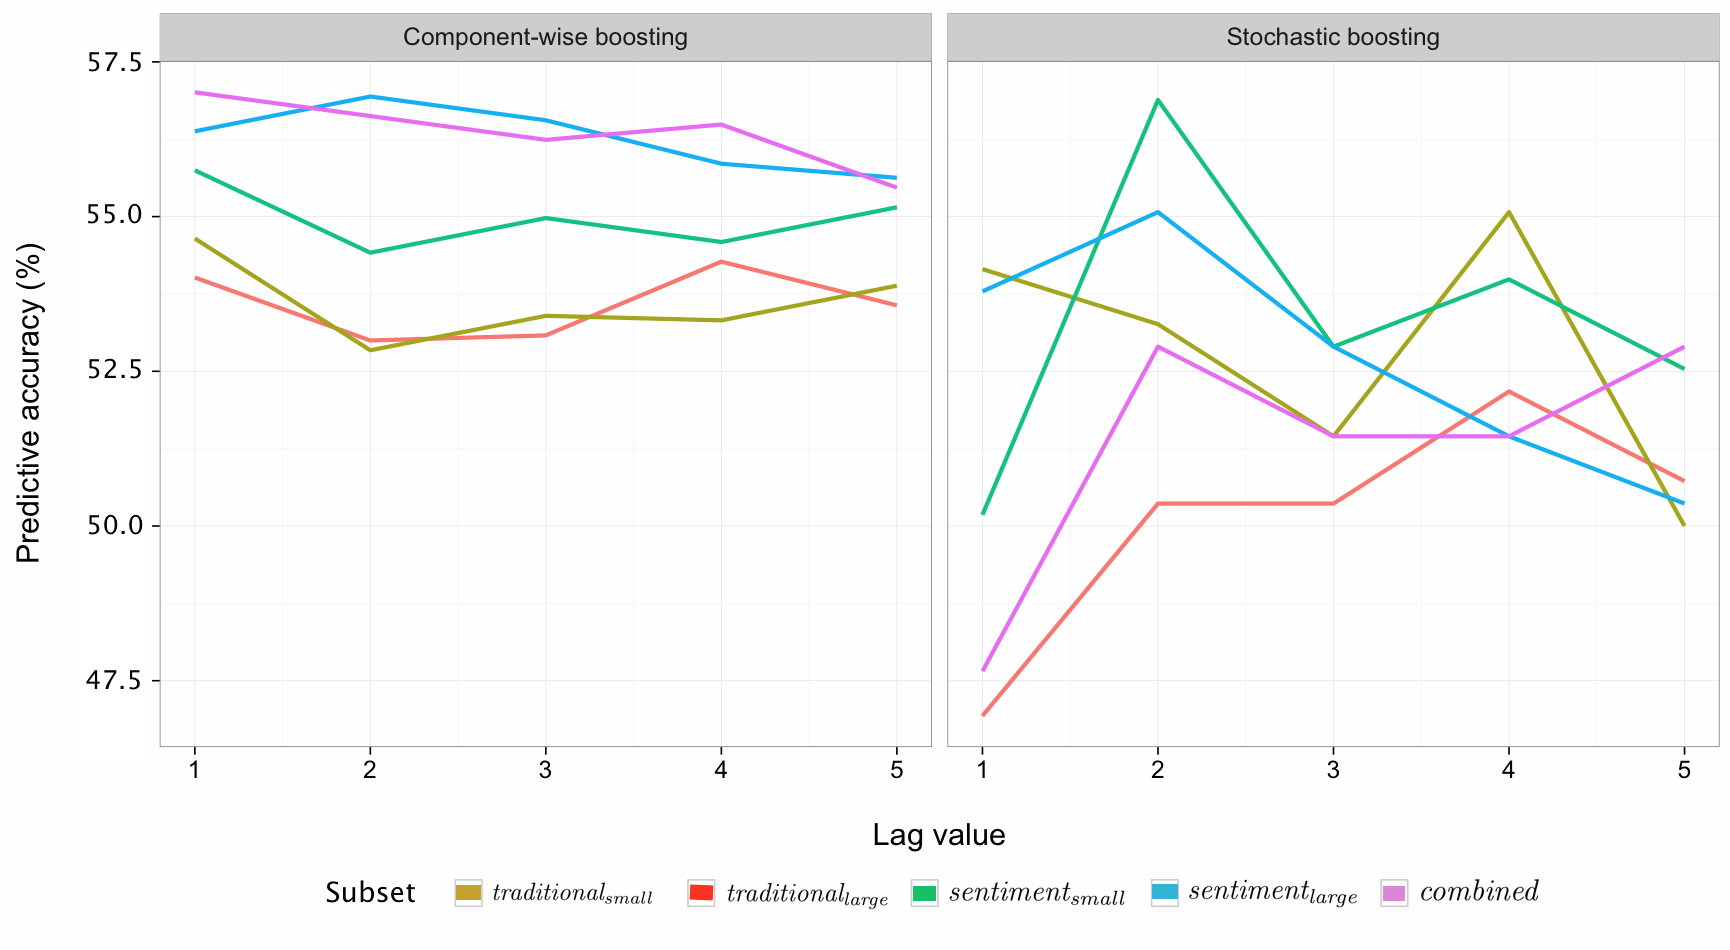
\includegraphics[width=16cm]{/Volumes/Mac OS Drive/Thesis/Source Code/Reporting/nwm_Report/images/stoch_boost.png}
\caption[The predictive accuracies of \emph{component-wise} versus \emph{batch} stochastic gradient boosting]{\label{fig:stoch-pred-acc}Predictive accuracies for component-wise boosting (left) are plotted alongside those using stochastic gradient boosting (right). Both results stem from identical input data sets, with pairwise correlation threshold, $\kappa$ = 80 \%.}
\end{figure}


\pagebreak

\vfill
\newpage
% Emacs 24.5.1 (Org mode 8.2.10)
\end{document}